% JuliaCon proceedings template
\documentclass{juliacon}
\setcounter{page}{1}

% --- additional packages (must appear before \begin{document}) ---
\usepackage{amsmath}
% never let a float be placed before its first reference in the text
\usepackage{flafter}
\hypersetup{hidelinks}

\begin{document}

% **************GENERATED FILE, DO NOT EDIT**************

\title{BeamletOptics.jl: Modeling optical setups with Gaussian beamlet propagation}

\author[1]{Hugo Uittenbosch}
\author[1]{Oliver Kliebisch}
\author[1]{Aurelius Manny}
\author[1]{Thomas Dekorsy}
\affil[1]{German Aerospace Center (DLR), Institute of Technical Physics, Stuttgart, Germany}

\keywords{Optical simulation, Ray tracing, Complex ray tracing, Gaussian beamlet tracing, Laser interferometry, Physical optics}

\hypersetup{
pdftitle = {BeamletOptics.jl: Modeling optical setups with Gaussian beamlet propagation},
pdfsubject = {JuliaCon 2025 Proceedings},
pdfauthor = {Hugo Uittenbosch, Oliver Kliebisch, Aurelius Manny, Thomas Dekorsy},
pdfkeywords = {Optical simulation, Ray tracing, Complex ray tracing, Gaussian beamlet tracing, Laser interferometry, Physical optics},
}



\maketitle

\begin{abstract}
Laying out an optical experiment on a breadboard, e.g. a laser
interferometer or a spectroscopy setup, is a common task for physicists
and optical engineers, yet the tooling to prototype such setups quickly
is either expensive, closed-source, or tied to the sequential surface
model of classical lens design software.

\textbf{BeamletOptics.jl} (BMO) is an open-source Julia package that
aims to fill this gap. It couples a 3D geometrical ray tracer with the
Complex ray and Gaussian beamlet formalisms,
so that the propagation of a laser beam through an arbitrarily
aligned arrangement of lenses, mirrors, beamsplitters and detectors can
be quickly investigated. Optical elements are modeled as closed volumes
described by meshes or signed distance functions. The underlying solver
calculates beam paths non-sequentially. Every component is freely
movable through a robust kinematic API. We describe the package
architecture, the ray and beamlet models it implements, showcase a 
Michelson interferometer example and validate the implementation against 
the analytical Fraunhofer diffraction pattern of a double slit.
\end{abstract}

\section{Introduction}

Before an optical setup is built on a laboratory breadboard, its
designer usually wants to answer a handful of practical engineering
questions. Will the beam fit through every aperture? Where does it come
to a focus, and how large is the waist there? What happens to the fringe
contrast of an interferometer when a mirror is tilted by a milliradian
or a mount drifts by a micron? Commercial optical design suites such as
Zemax OpticStudio, CODE~V or FRED can answer these questions, but they
are costly and closed source. An open-source alternative is therefore
attractive, and the Julia programming language \cite{bezanson2017julia}
offers a variety of in-built features, such as performance, automatic
differentiation (AD) and easy access to multi-threading, that allow for
rapid iteration of algorithms.

BMO is being developed at the Institute of Technical Physics (DLR), where one
of the motivating applications is the design of heterodyne laser
interferometers for two-color pressure measurement
\cite{Uittenbosch2023}. In that context a \emph{digital twin} of the
planned laboratory setup becomes relevant: a model that predicts, for
instance, the interferometric phase and contrast as components are moved
or perturbed, in the spirit of the mission-grade simulators built for
space gravitational-wave detectors \cite{Wanner:2017}, but lightweight
enough to iterate on rapidly \cite{Manny:2024}. Since many of these
experiments use laser beams in the fundamental transverse
electromagnetic ($\mathrm{TEM}_{00}$) mode, utilizing the Gaussian
beamlet formalism offers a performant tool for the design and analysis
of optical setups. This method builds upon geometrical optics and ray
tracing, which are established techniques.

Within the Julia ecosystem several optics packages already exist, each
with a different scope. \texttt{OpticSim.jl} \cite{Guenter2021} is a
full sequential/non-sequential lens design and optimization framework
built on constructive solid geometry. \texttt{ABCDMatrixOptics.jl}
\cite{ABCDMatrixOptics} implements the paraxial ray-transfer-matrix
($ABCD$) formalism for Gaussian beams in 2D.
\texttt{WaveOpticsPropagation.jl} \cite{WaveOpticsPropagation} performs
scalar diffraction propagation of sampled fields. What has been missing
is a lightweight tool aimed specifically at \emph{prototyping}
three-dimensional breadboard setups with laser sources: one that
does not assume a fixed optical axis or surface order, lets the user
move components interactively, and provides the physical-optics
quantities (waist, curvature, phase, interference) that matter for a
coherent source.

In Fig.~\ref{fig:openraman} the kind of setup that BMO targets is displayed. 
The OpenRAMAN spectrometer \cite{OpenRAMAN} is traced using a
laser beam model for the excitation path and geometrical ray tracing for
the Raman scattering path.

\begin{figure}[h]
% trim is in bp; the PNG is 2400x1600 px at 192 dpi, i.e. 900x600 bp,
% so 1 bp = 8/3 px. Values below strip the white margin only.
\centerline{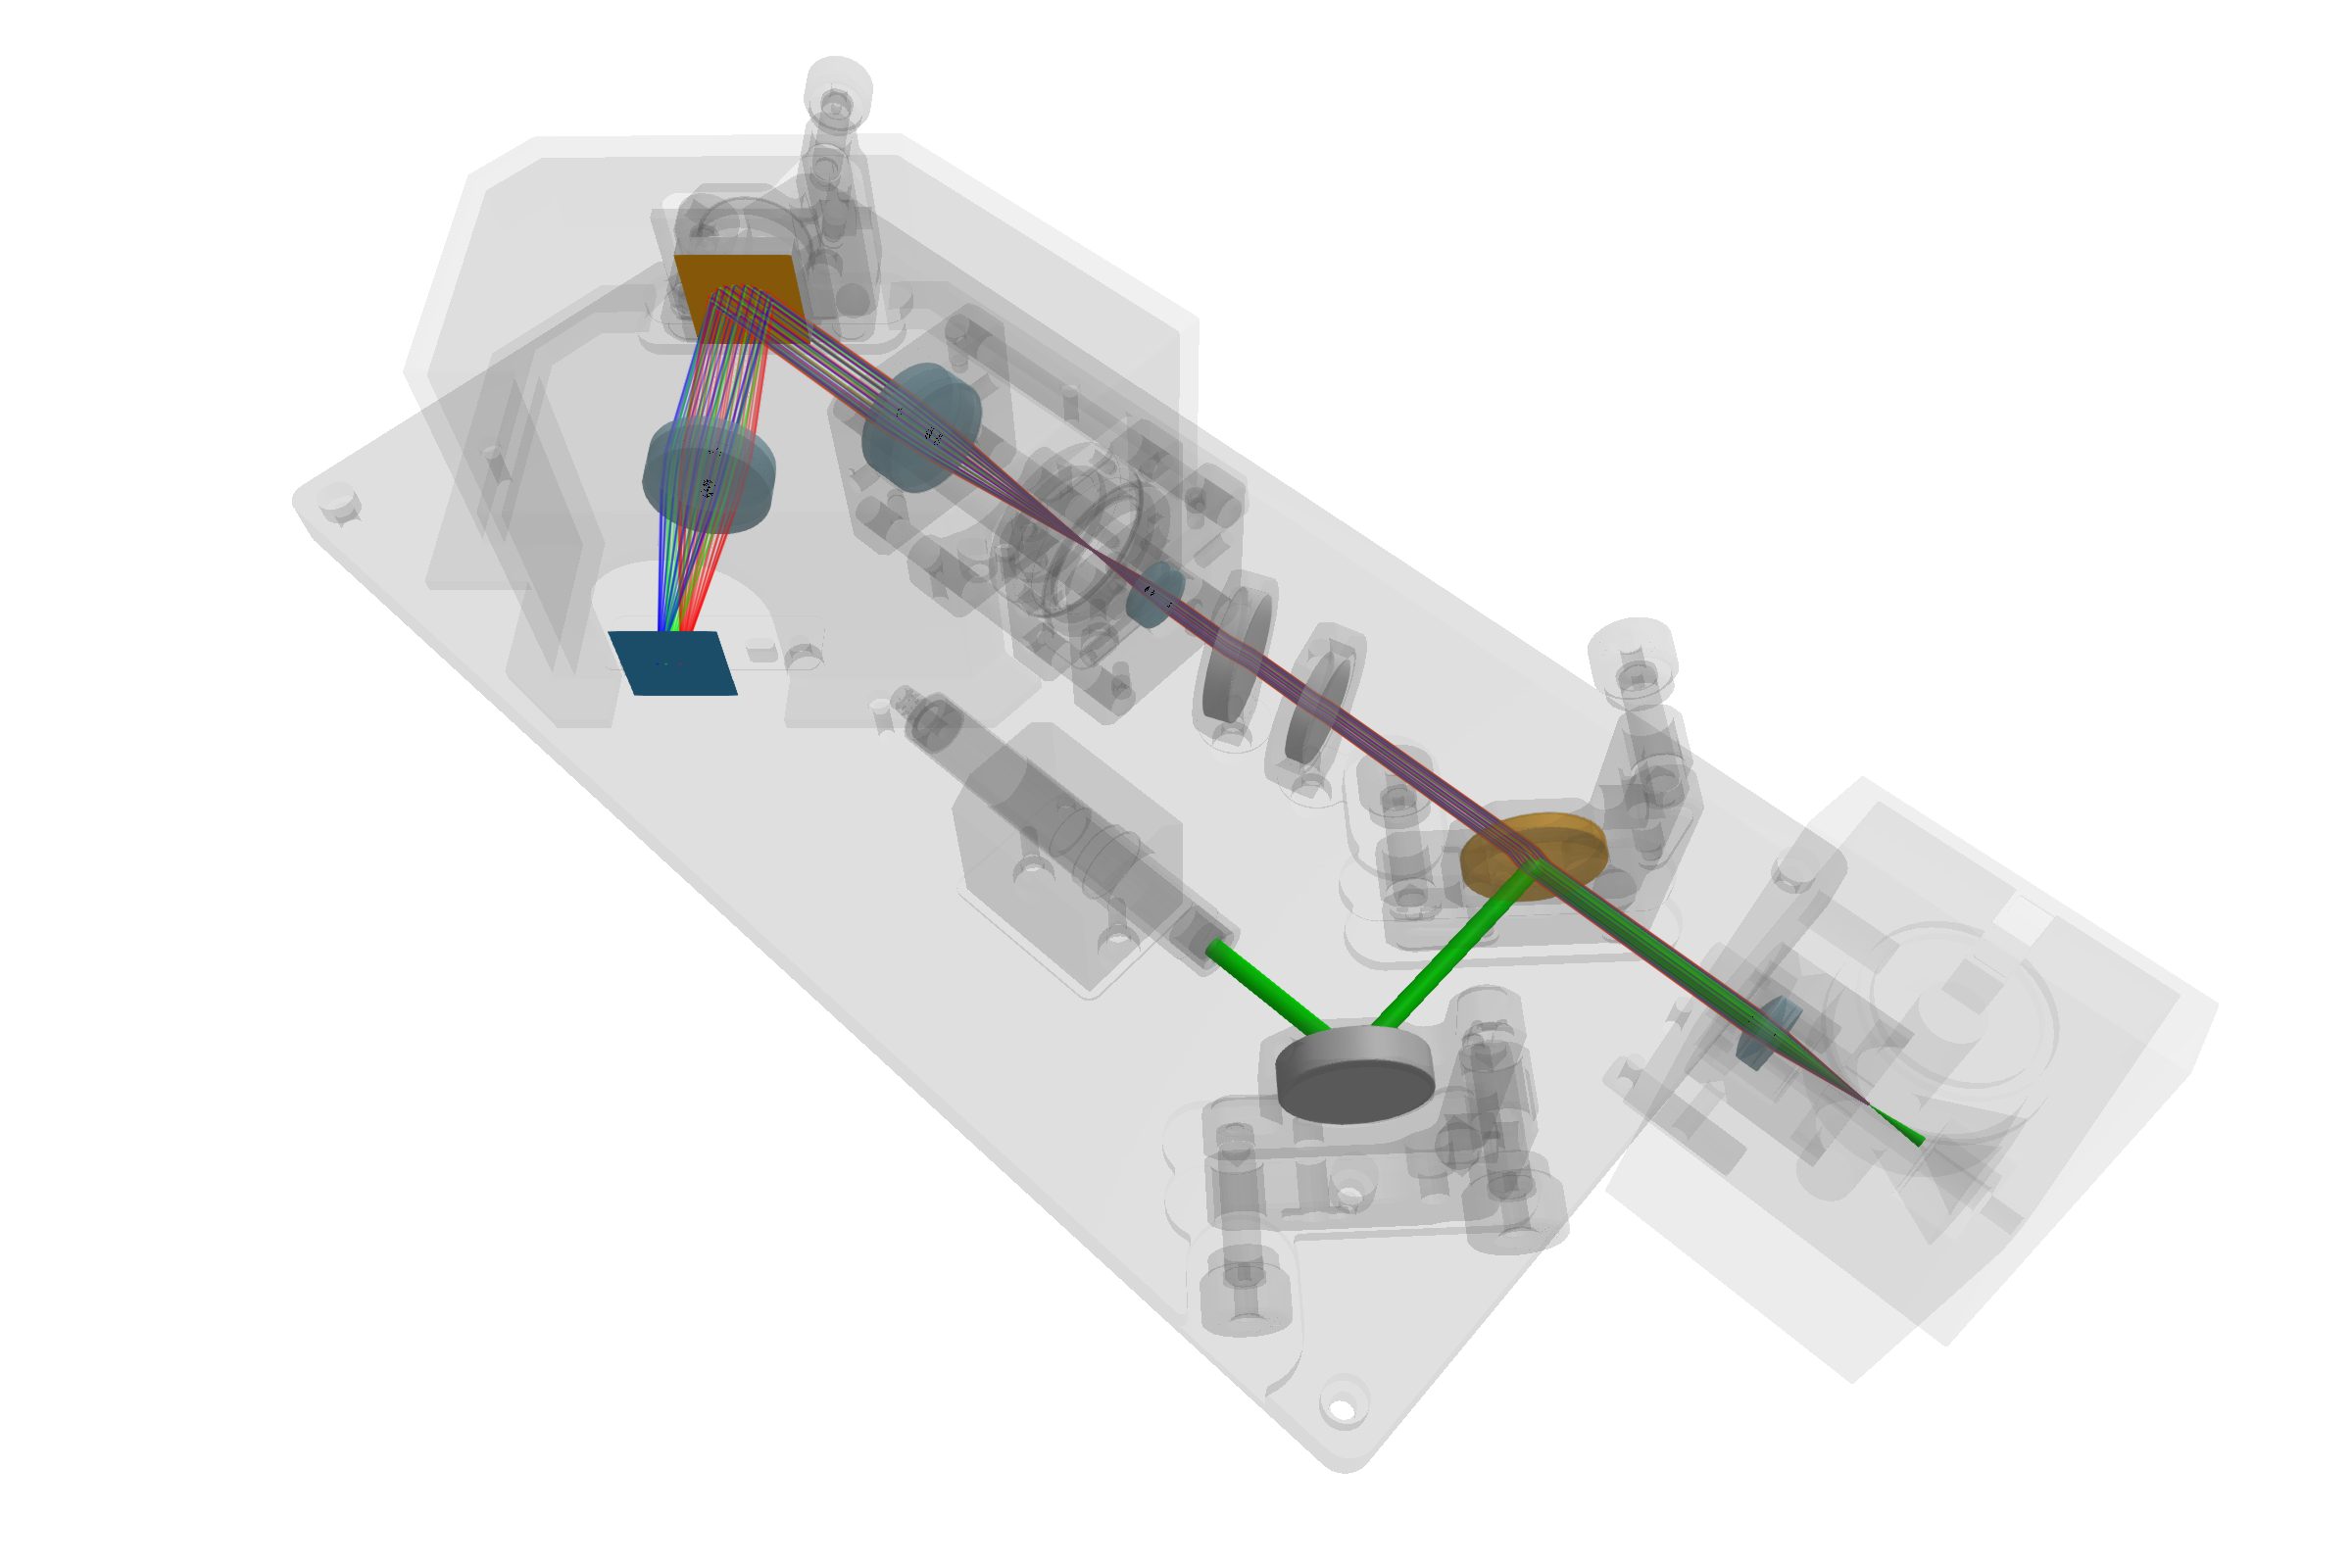
\includegraphics[trim=100 10 35 10, clip,
width=\columnwidth]{figures/openraman.png}}
\caption{OpenRAMAN spectrometer BMO model. The excitation light
(green) is folded through the
instrument, and the returning signal is traced at several wavelengths
(coloured) through the collection optics onto the sensor plane (blue).
The housing and opto-mechanical mounts are imported as meshes and
included as non-interacting geometry so that beam clearance can be
inspected in the same scene as the optical path.}
\label{fig:openraman}
\end{figure}

BMO is registered in the Julia General registry, released under the MIT
license, and archived on Zenodo \cite{BeamletOptics_zenodo}. This paper
describes the tagged version \texttt{0.13}. The design goals, in order
of priority, are:
\begin{enumerate}
  \item \emph{Prototyping speed over optimization.} BMO is intended
  primarily as a digital
breadboard simulator, not a lens optimizer. It deliberately offers no
in-built support for optimization, but allows users to integrate tools
from the Julia ecosystem, e.g. \texttt{Optimization.jl}
\cite{Optimization_jl}, based on custom merit functions.
  \item \emph{Robust kinematics.} Every component can be translated and
rotated in 3D between solver calls, enabling the simulation of e.g.
alignment or vibrations.
  \item \emph{Physical-optics output for lasers.} The $\mathrm{TEM}_{00}$
Gaussian mode is useful to represent many lasers used in optical setups.
BMO offers easy access to beam models that allow simulating coherent
laser sources.
  \item \emph{Geometry-agnostic solving.} Optical interactions are
decoupled from their geometric representation, so that surfaces, meshes
and signed distance functions can coexist and be extended independently
in the future.
\end{enumerate}

\section{A minimal example}

Code~\ref{lst:expander} builds a Keplerian beam expander from two stock
spherical lenses and traces a bundle of collimated rays through it. It
shows the three steps of every BMO simulation: constructing
components, placing them with the kinematic API, and calling
\texttt{solve\_system!}. The result is illustrated in
Fig.~\ref{fig:expander}. The paraxial rays emerge collimated and
magnified by $M = f_2/f_1$, while rays sent through the lens margins
focus short of the axis. Spherical aberrations appear directly from the
exact, non-paraxial surface trace, with no aberration model added.

\begin{lstlisting}[
  language = Julia,
  numbers = left,
  float = h,
  label = {lst:expander},
  caption = {A two-lens Keplerian beam expander. Visualization becomes
available once a Makie backend is loaded, examples can be found in the BMO documentation.}
]
  using BeamletOptics
  # two thin spherical lenses, n = 1.5 for all λ
  l1 = SphericalLens(
    20e-3,    # front side radius of curvature
    60e-3,    # back side radius of curvature
    0,        # cylinder section thickness
    25.4e-3,  # lens diameter
    λ -> 1.5  # dispersion mapping
  )
  l2 = SphericalLens(60e-3, 90e-3, 0,
    50.8e-3, λ -> 1.5)

  system = System([l1, l2])
  zrotate3d!(l1, pi); zrotate3d!(l2, pi)
  # confocal spacing
  f1, f2 = 24e-3, 72e-3 # from lensmaker's eq.
  translate3d!(l2, [0, f1 + f2, 0])
  # collimated ray fan
  for z in -8e-3:2e-3:8e-3
    beam = Beam(Ray([0, -0.15,z], [0, 1.0, 0]))
    solve_system!(system, beam)
  end
\end{lstlisting}

\begin{figure}[h]
% trim in bp; the PNG is 2400x960 px at 384 dpi, i.e. 450x180 bp,
% so 1 bp = 16/3 px. Values below strip the white margin only.
\centerline{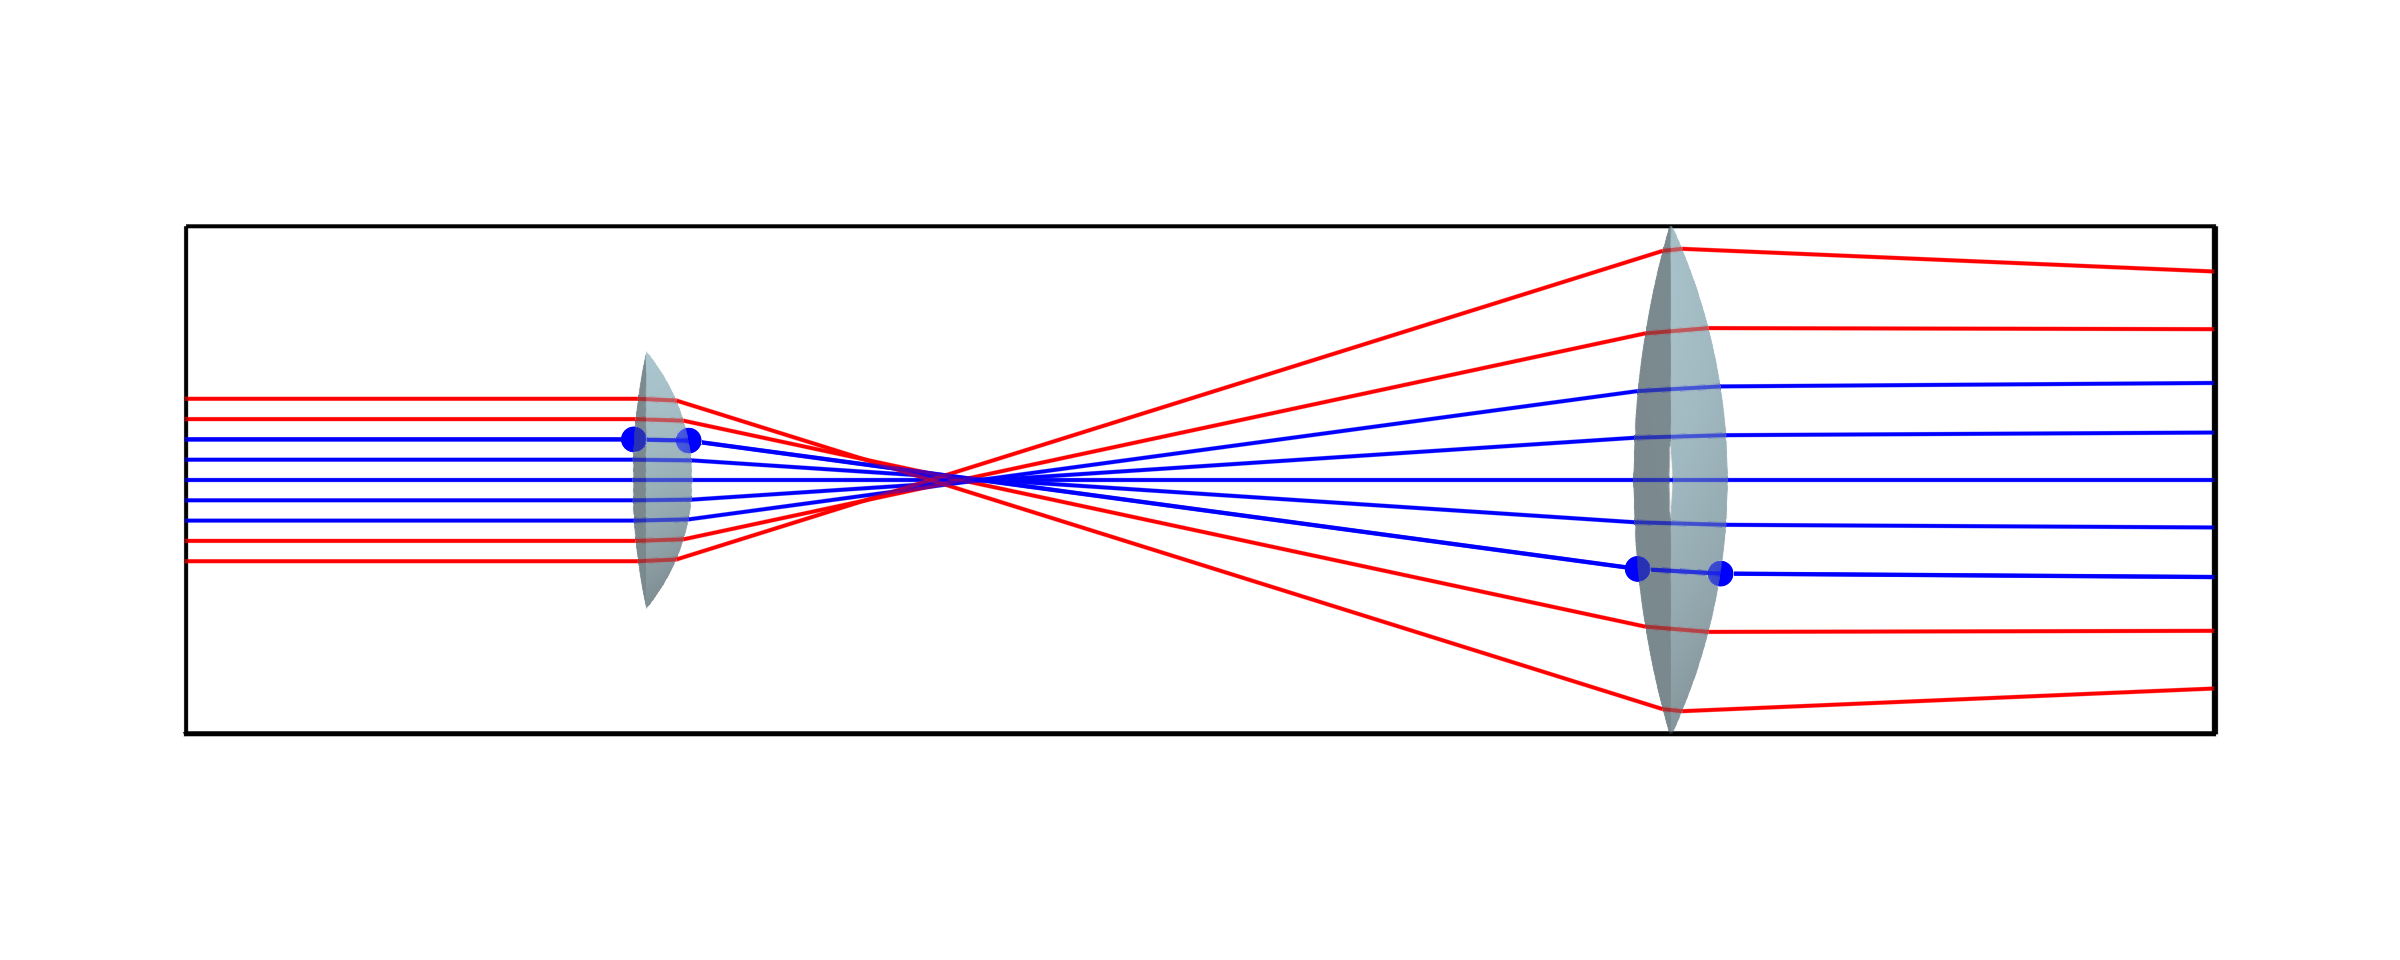
\includegraphics[trim=32 38 30 38, clip,
width=\columnwidth]{figures/expander_aberrations.png}}
\caption{Geometrical ray trace of the beam expander in
Code~\ref{lst:expander}. Paraxial rays (blue) emerge collimated and
magnified; marginal rays (red) are under-corrected, i.e. spherical
aberration. For one ray, the surface intersection points have been
marked (blue dots).}
\label{fig:expander}
\end{figure}

\section{Package architecture}

\subsection{Objects and shapes}

The BMO architecture distinguishes between an optical \emph{object},
i.e. how light interacts when it meets an element, and its \emph{shape},
referring to the 3D representation in space. An \texttt{AbstractObject}
owns one or more \texttt{AbstractShape}s and an \texttt{interact3d}
method; an \texttt{AbstractShape} owns an \texttt{intersect3d} method
and nothing else. This separation means the same \texttt{Lens}
interaction logic applies whether the lens body is a triangulated mesh
or an implicit surface, and new geometry backends (e.g. boundary
representation) can be added without touching the optic models.

Unlike classical surface-based tracers, BMO treats every optical element
as a closed volume. A lens, for instance, is a dielectric body bounded
by a closed refracting shell, not a collection of (independent)
surfaces. A plate beamsplitter is a substrate with a coating on one
face. Closed volumes remove the ambiguity of ``which side am I on'' for
a ray that starts exactly on an interface, and they make non-sequential
tracing robust for arbitrary angles of incidence. Composite elements
like cemented doublets, prisms and cube beamsplitters can be defined by
assigning the \texttt{MultiShape} trait and are assembled from
sub-volumes or even sub-objects. Where two such sub-volumes touch, the
solver needs additional information to resolve which of them a ray is
leaving; how this is supplied is covered in Section~\ref{sec:nonseq}.

\subsection{Signed distance functions and ray marching}

Curved surfaces in BMO are represented by \emph{signed distance
functions} (SDFs): a function that maps a point in $\mathbb{R}^3$ to the
signed distance to the nearest surface, negative inside the volume
\cite{Osher:2003}. This is necessary because tessellated surfaces do not
offer the surface normal accuracy that optical ray tracing demands.
Ray--surface intersection is then performed by \emph{sphere tracing}
\cite{Hart1996}: starting from the ray origin, the SDF is evaluated and
the ray advanced by that (guaranteed safe) distance, repeating until the
distance falls below a tolerance or the ray escapes
(Fig.~\ref{fig:spheretracing}). The scheme has three properties that
matter for optics:
\begin{enumerate}
  \item \emph{SDF generalizability.} The intersection point is found to
arbitrary precision by simple iteration, with no surface-specific solver
required.
  \item \emph{Surface normal accuracy.} The surface normal, on which
every refraction and reflection calculation depends, is obtained exactly
by automatic differentiation of the SDF \cite{Revels2016}, or
numerically when the SDF is non-exact \cite{Quilez_sdf}.
  \item \emph{Ray marching.} The same ray marching loop works for any
shape that supplies an SDF, including composite SDFs. This lowers the
maintenance burden.
\end{enumerate}

\begin{figure}[t]
\centerline{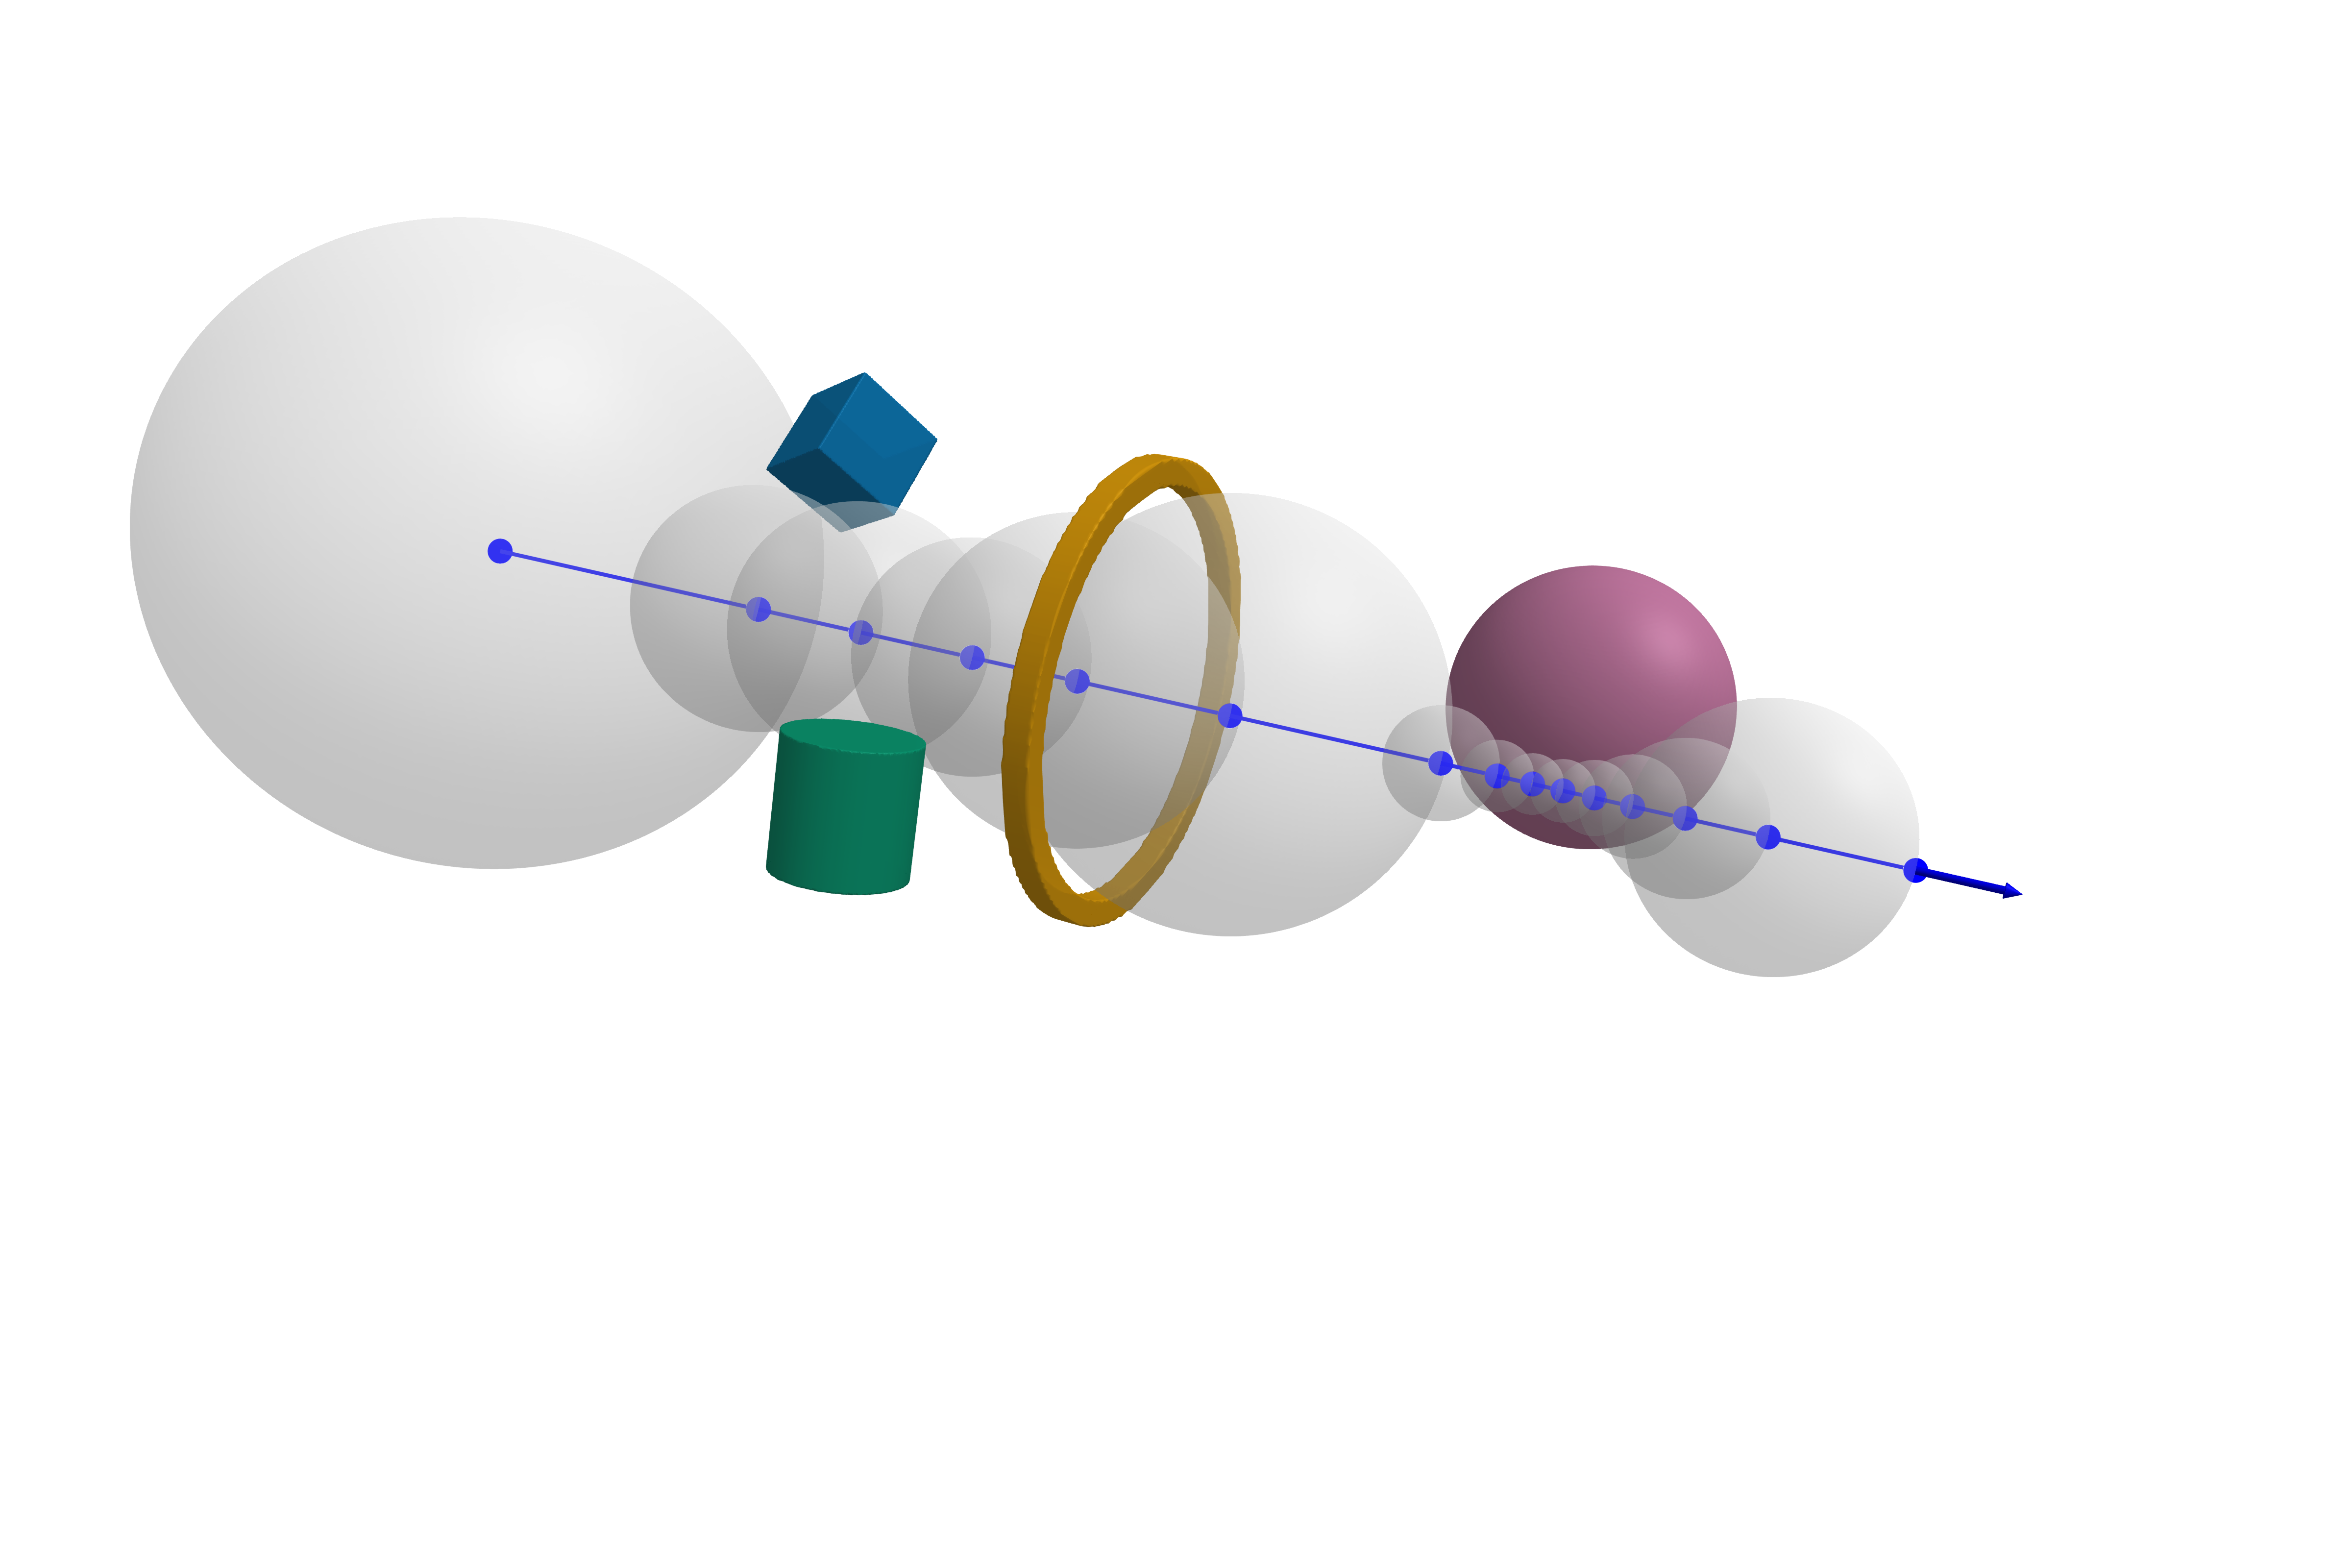
\includegraphics[width=\columnwidth]{figures/sphere_tracing.png}}
\caption{Sphere tracing through a scene of SDF primitives. At each
iteration the SDF gives the distance to the nearest surface, drawn here
as a translucent sphere: the ray may advance by that radius without
tunnelling through geometry. Steps are large in open space and shrink as
the ray approaches a surface.}
\label{fig:spheretracing}
\end{figure}
Lens volumes are composed from Quilez's analytic primitives
\cite{Quilez_sdf}, e.g. cut spheres or cylinders, and joined by a
boolean union (\texttt{UnionSDF}), which stays exact under addition. On
top of these, iterative root-finding routines extend the marcher to
rotationally-symmetric even aspheres (ISO~10110) and (a)cylindrical
lenses. SDFs are established in computer graphics and have been used for
radiative transfer in curved geometries \cite{McMillan:2022}. Their use
as the primary geometry backend of an optical ray tracer is, to our
knowledge, new. For flat surfaces and imported CAD geometry BMO also
provides a mesh backend using the M\"oller--Trumbore intersection
algorithm \cite{Moeller:2005}, but with a constant normal vector for each face it is
unsuitable for curved optical surfaces and intended mainly for
visualization and placeholder optomechanics.

\subsection{The Intersect--Interact--Repeat loop}

Solving a system means calling \texttt{solve\_system!(system, beam)}.
Internally this runs the \emph{Intersect--Interact--Repeat} loop
sketched in Fig.~\ref{fig:iir}:

\begin{enumerate}
  \item \textbf{Intersect}: find the closest intersection between the
current ray and any shape in the system.
  \item \textbf{Interact}: evaluate \texttt{interact3d} at that surface
or within that volume to produce the next ray segment (refraction,
reflection, splitting, absorption, \ldots).
  \item \textbf{Repeat}: append the new segment to the beam tree and go
back to step~1, until the ray escapes or a recursion limit is hit.
\end{enumerate}
The fidelity of a simulation is limited only by how much information
\texttt{interact3d} is given; a user can add a new optical effect by
defining a new method of this function for their object and ray types,
without modifying the solver.


\begin{figure}[t]
\centerline{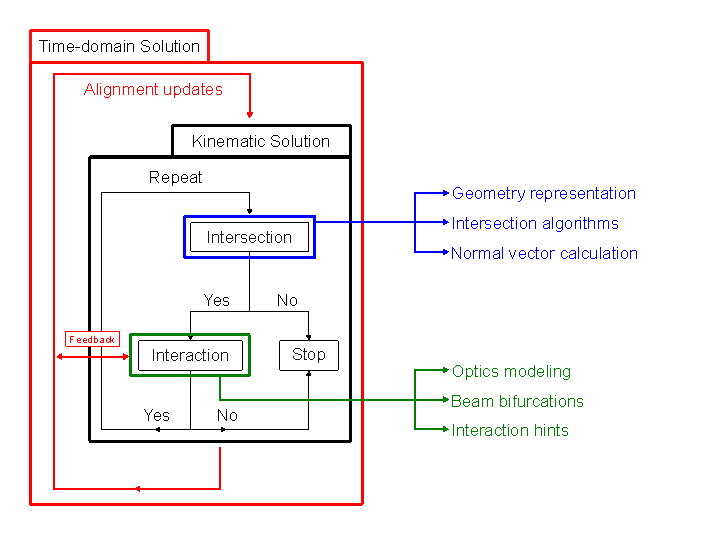
\includegraphics[width=\columnwidth]{figures/iir_loop.pdf}}
\caption{The Intersect--Interact--Repeat loop. The inner black loop represents
the static ray trace; the outer red loop is the time-domain solution, in
which component alignment is updated between successive
\texttt{solve\_system!} calls. Blue and green annotations mark the two
extension points: the geometry backend supplying intersections and
normals, and the optics model supplying \texttt{interact3d}, beam
bifurcations and hints.}
\label{fig:iir}
\end{figure}

\subsection{Non-sequential tracing}
\label{sec:nonseq}

In general, BMO traces non-sequentially: each ray is tested against
every element in the system, and the order in which components were
added to the \texttt{System} is irrelevant. Nothing about the beam path
needs to be declared in advance, which is what allows components to be
moved freely and systems to be assembled without specifying a surface
sequence. The price is that the intersection search scales linearly with
the element count, as in $\mathcal{O}(n)$.

Where knowledge about the next relevant object is available, it can be
handed to the solver through the \texttt{Hint} interface, which
short-circuits the search by naming the object/shape to test next. This
is a general mechanism, but it is what makes multi-shape objects
possible in the first place: at the internal interface of a cemented
doublet or a plate beamsplitter a ray starts exactly on the boundary
between two shapes, and deciding which of them to test next from the
local geometry alone is possible, but tends to require a good deal of
special-case code. Handing the solver a hint is how BMO resolves this
currently. The hint travels back to the solver as part of the
interaction returned by \texttt{interact3d}, so supplying a correct one
is the responsibility of whoever implements such a composite element.
Systems without mutable elements can be marked as \texttt{StaticSystem} for
more aggressive compiler specialization, and independent rays are traced
in parallel on the CPU.

\subsection{Kinematic API}

Every object exposes a \texttt{position} (an $\mathbb{R}^3$ centroid)
and an \texttt{orientation} (an orthonormal $3\times3$ matrix). Relative
moves are made with \texttt{translate3d!}, \texttt{rotate3d!} and 
axis-specific helpers, e.g. \texttt{zrotate3d!}. Components can be
locked together in an \texttt{ObjectGroup} that moves rigidly, which is
how multi-element lens assemblies and zoom groups are built. All
coordinate systems are right-handed and rotations are
counter-clockwise-positive. A notable difference with respect to common
definitions is the use of the global $y$-axis as the initial optical
axis of some elements. This definition was chosen to match the one often
used in CAD programs or Makie \cite{Danisch2021}, in which the $x$--$y$
plane is the horizontal plane.

\section{Light propagation models}

\subsection{Rays and beams}
\label{sec:rays}

The basic carrier of optical information is a ray
$\vec{x}(t) = \vec{p} + t\,\vec{d}$ with position $\vec{p}$ and unit
direction $\vec{d}$, valid between its origin and the next intersection.
A \texttt{Ray} reflects and refracts according to the vector form of
reflection and Snell's law \cite{Spencer1962}, respectively. A
\texttt{Beam} stores the resulting chain of segments
(Fig.~\ref{fig:beam}) as an \texttt{AbstractTrees.jl}-compatible tree
\cite{AbstractTrees}, so that a beamsplitter can attach two children to
the segment at which the parent path terminates. To model polarizing
elements a \texttt{PolarizedRay} additionally carries the complex
$\mathbb{R}^3$ electric field vector and propagates it with the
three-dimensional polarization ray-tracing calculus of Yun et al.
\cite{Yun2011_1, Yun2011_2}, a 3D generalization of the Jones calculus.
The amplitude coefficients at each interface follow the Fresnel
equations with the sign convention of Fowles \cite{Fowles1989} and
Peatross \cite{Peatross2015}, including total internal reflection.
Idealized Jones elements (linear polarizers, and, in progress, wave
plates and rotators) are also available, with oblique incidence handled
by projection into the transverse plane \cite{Korger2013}.

\begin{figure}[h]
\centerline{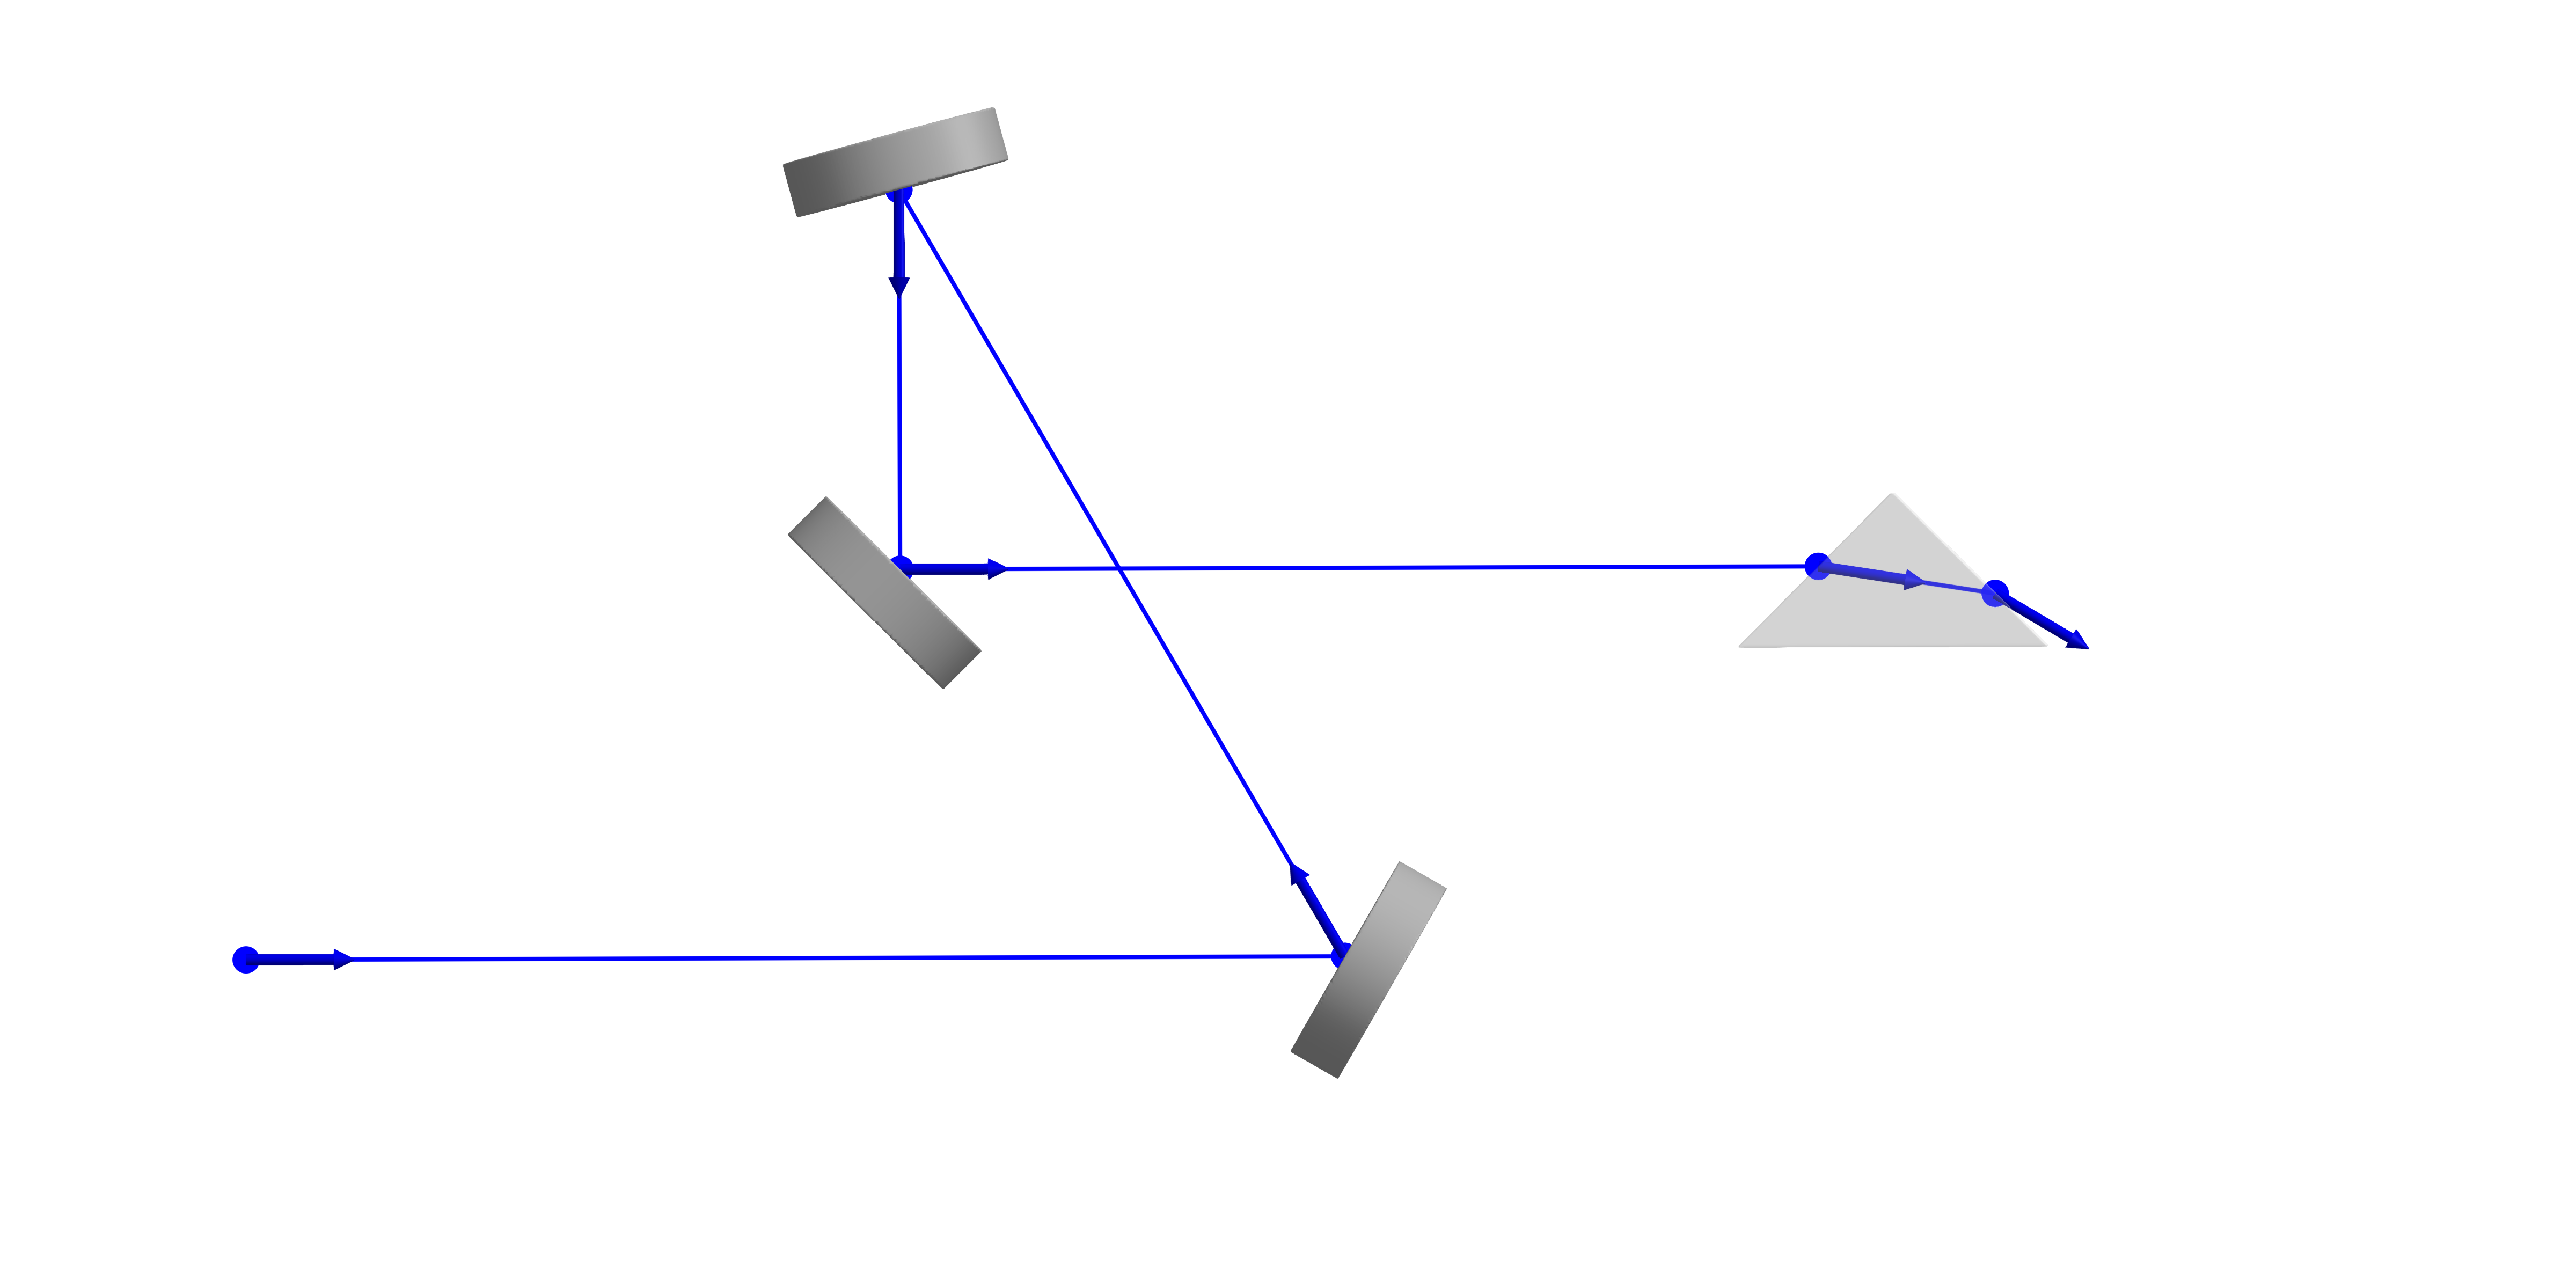
\includegraphics[width=\columnwidth]{figures/beam_showcase.png}}
\caption{A \texttt{Beam} traced through plano mirrors and a right-angle
prism. Each \texttt{Ray} segment stores its origin (dot) and unit
direction (arrow); the chain is built one segment at a time by the
Intersect--Interact--Repeat loop and ends when the last ray leaves the
system.}
\label{fig:beam}
\end{figure}

\subsection{Stigmatic Gaussian beamlets}

Geometrical rays can not by themselves describe the Gaussian mode of a laser, 
whose radius, wavefront curvature and Gouy phase evolve according to wave optics \cite{Saleh2019}.
One method for Gaussian propagation already implemented as a Julia package is the $ABCD$
$q$-parameter method \cite{ABCDMatrixOptics}, which requires a paraxial
system matrix. BMO instead uses the \emph{complex ray} method introduced 
by Arnaud \cite{Arnaud1968}: a fundamental Gaussian can be represented by 
a small number of ordinary geometrical rays traced through the optical system.

The \texttt{GaussianBeamlet} represents the $\mathrm{TEM}_{00}$ mode with three coplanar
rays (Fig.~\ref{fig:beamlet}). A \emph{chief} ray along the axis, a
\emph{waist} ray offset by $w_0$, and a \emph{divergence} ray tilted by
the far-field half-angle
\begin{equation}
\theta = \frac{M^2 \lambda}{\pi w_0},
  \label{eq:divergence}
\end{equation}
where $M^2 \geq 1$ is the beam quality factor and $\lambda$ the wavelength. After tracing all three
rays through the system, the local beam radius $w(z)$, radius of
curvature $R(z)$ and Gouy phase $\psi(z)$ are reconstructed in cylinder coordinates $(r,z)$ 
from the ray heights and slopes using the relations of Herloski \cite{Herloski1983}
and DeJager \cite{DeJager1992}. The complex field of the mode is then
\begin{equation}
  \begin{split}
    E(r,z) = {}& E_0\,\frac{w_0}{w(z)}
      \exp\!\left(-\frac{r^2}{w(z)^2}\right) \\
      &\cdot \exp\!\left(i\left[kz + \psi(z)
        + \frac{k r^2}{2 R(z)}\right]\right),
  \end{split}
  \label{eq:gaussfield}
\end{equation}
with $k = 2\pi/\lambda$ being the wavenumber. In addition, the optical path length of the
chief ray is tracked so that the absolute phase of interfering beams is
correct. This model is exact for a mode that stays on axis and meets
only locally parabolic or flat surfaces; it does not capture
astigmatism, spherical aberration or polarization aberration, and the
beam can not be clipped by hard apertures. Within
these limits it is cheap, i.e. three rays per beam, and yields $w$, $R$
and $\psi$ directly, which makes it a good default for first-order
layout work; the astigmatic model of the next section covers the cases
it can not.

\begin{figure}[h]
\centerline{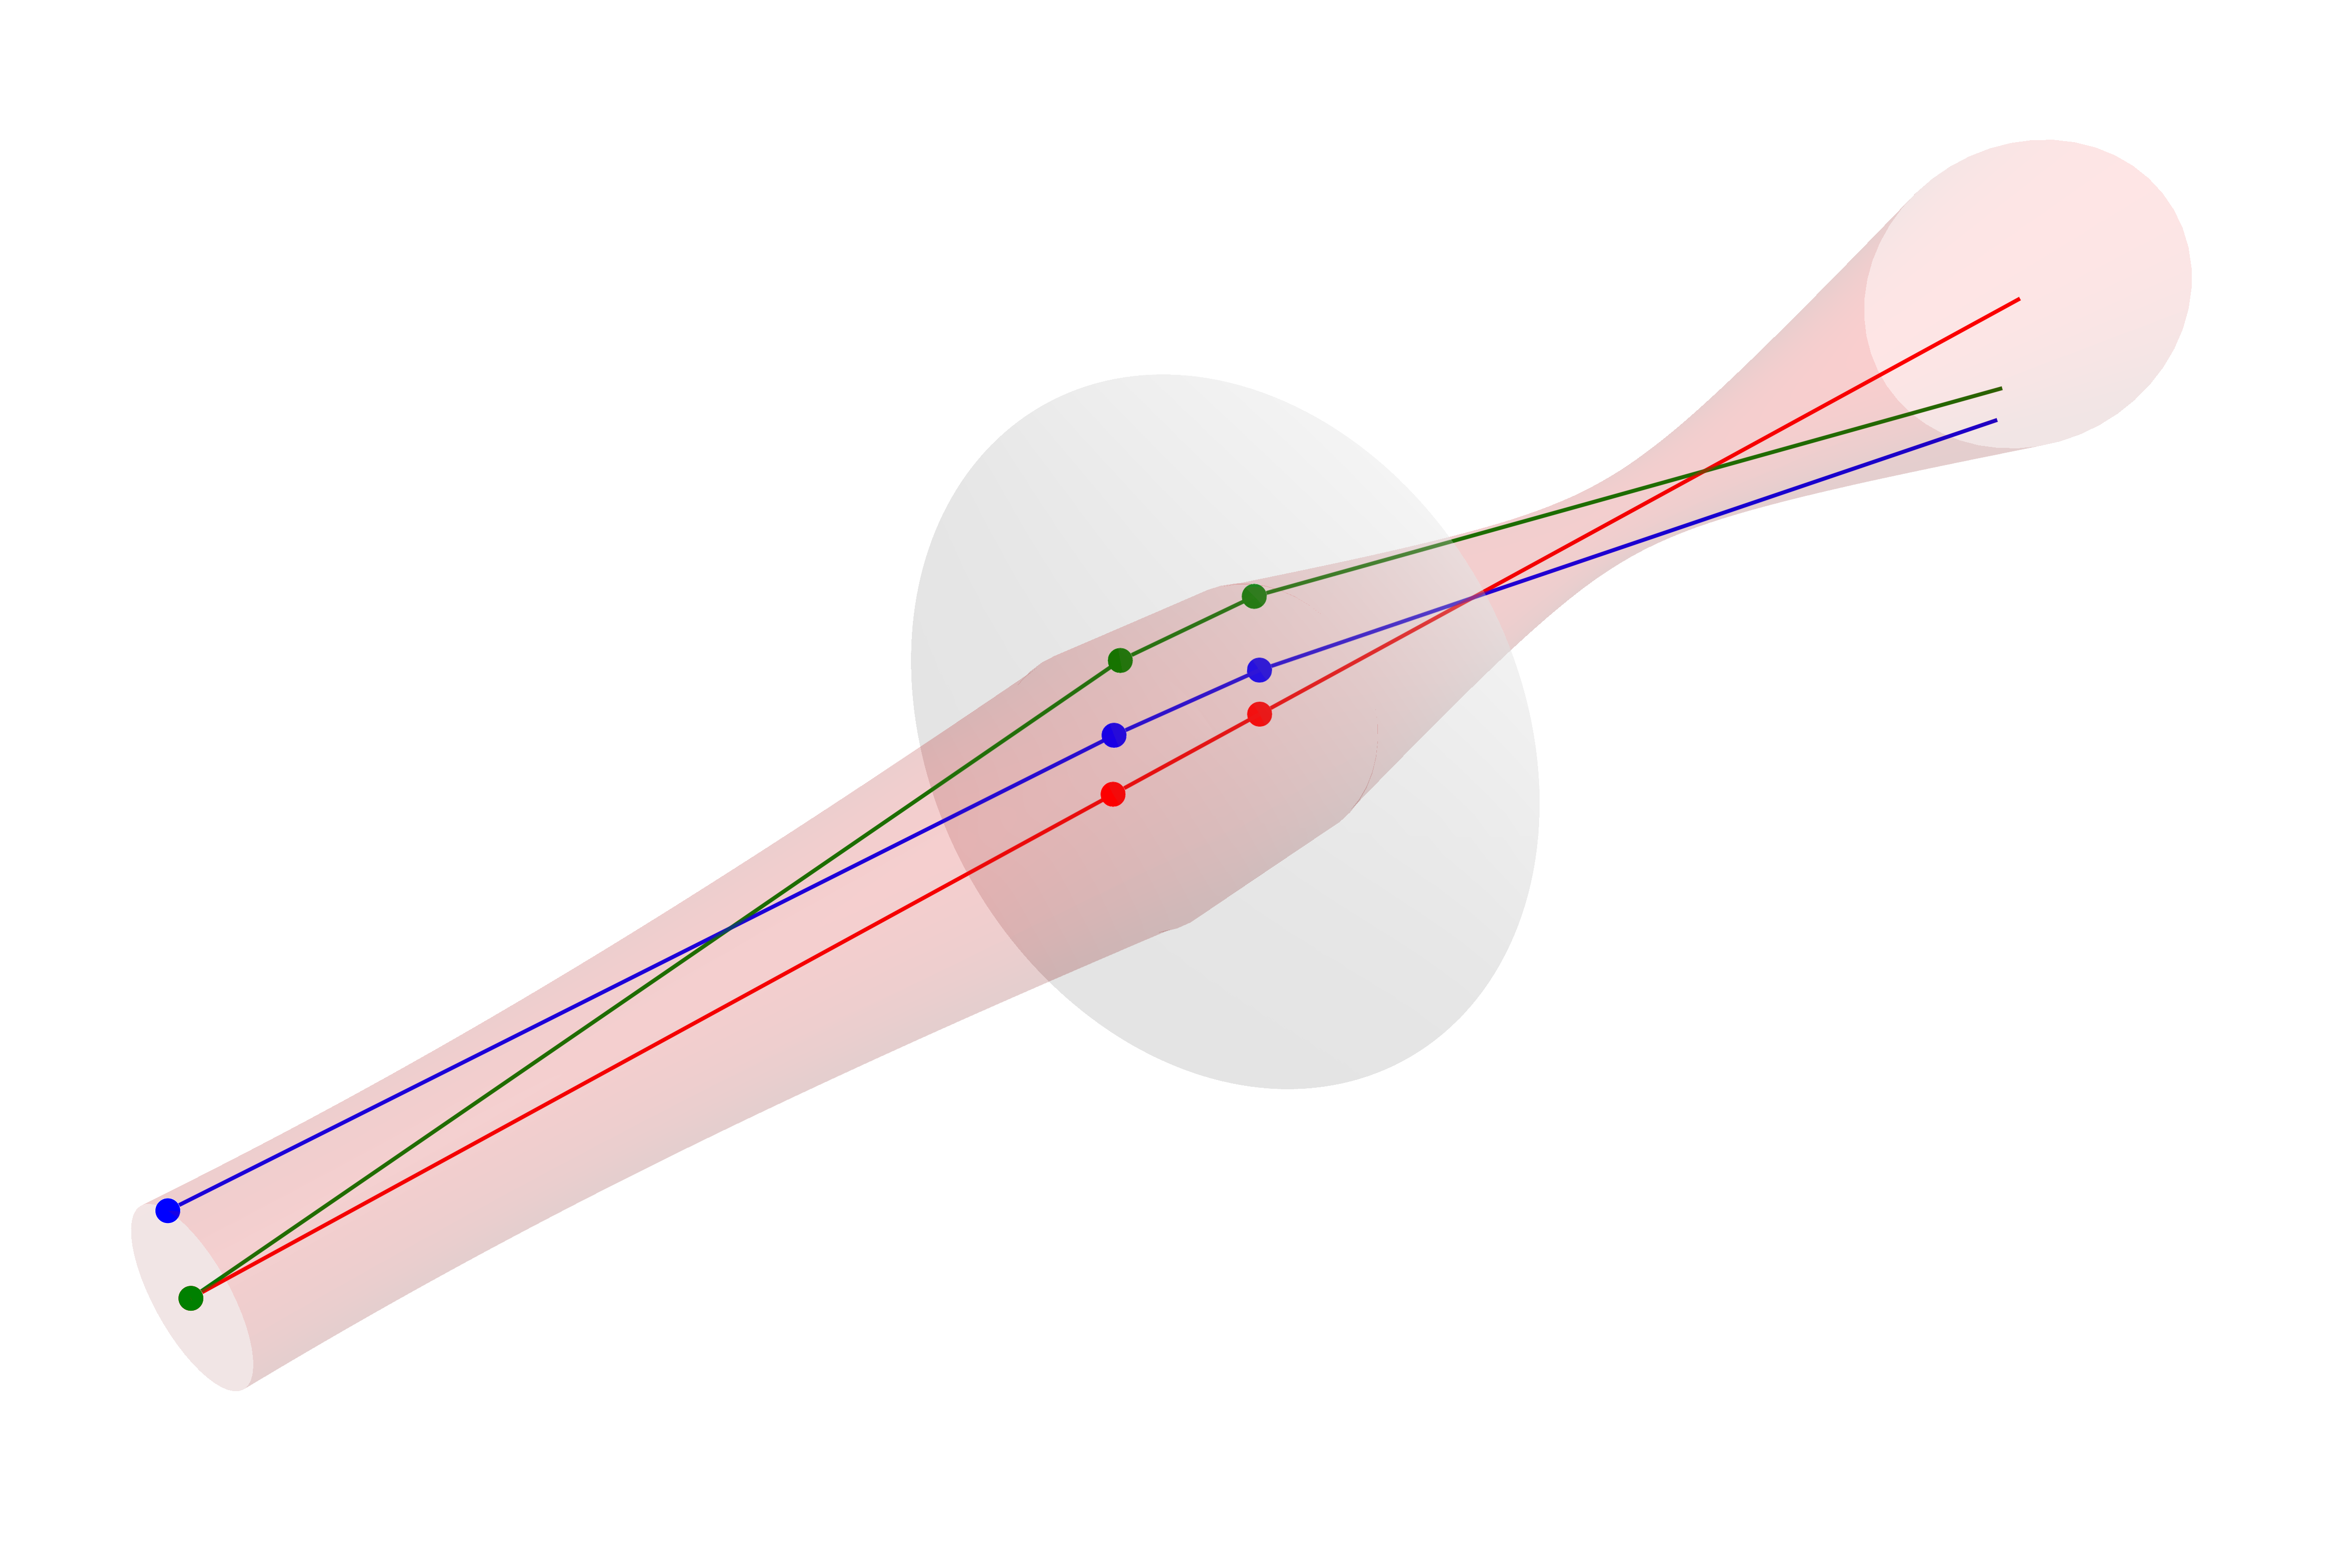
\includegraphics[width=\columnwidth]{figures/gaussian_showcase.png}}
\caption{A \texttt{GaussianBeamlet} focused by a single lens. The $\mathrm{TEM}_{00}$ mode
is carried by three geometrical rays: chief (red), waist (blue) and
divergence (green). From their heights and slopes the $1/e^2$ envelope
shown in red, together with $w(z)$, $R(z)$ and $\psi(z)$, is
reconstructed using the relations of Herloski \cite{Herloski1983} and
DeJager \cite{DeJager1992}.}
\label{fig:beamlet}
\end{figure}

\subsection{Astigmatic polarized Gaussian beamlets}

For off-axis or non-symmetric optical systems, a stigmatic beam
model is generally insufficient \cite{Kochkina:2013}.
BMO therefore provides the \texttt{AstigmaticGaussianBeamlet}, based on the generally
astigmatic formalism of Greynolds \cite{Greynolds:1986_1, Greynolds:1986_2}
and its polarization-aware formulation by Worku and Gross \cite{Worku:2017}.
Each beamlet is comprised of a polarized chief ray and eight auxiliary
rays: two positive and negative waist pairs and two divergence ray pairs along two
orthogonal transverse directions. Refer to Fig.~\ref{fig:agbeamlet} for a visual breakdown.
The following mathematical description for the field reconstruction from a traced set of rays 
assumes a fundamental Gaussian mode with $M^2=1$.

At each evaluation plane perpendicular to the chief-ray direction
$\hat{\mathbf d}$, the auxiliary rays define two complex height
vectors $\mathbf h_1,\mathbf h_2$ and two complex direction
vectors $\mathbf u_1,\mathbf u_2$.
BMO constructs their real parts from the waist-ray pairs and
their imaginary parts from the divergence-ray pairs, using half
the difference between the positive and negative rays.

Expressed in a common orthonormal transverse basis, these vectors
form the matrices
\[
    H = [\mathbf h_1,\mathbf h_2],
    \qquad
    U = [\mathbf u_1,\mathbf u_2],
    \qquad
    Q = UH^{-1}.
\]
The complex curvature matrix $Q$ determines the transverse
quadratic phase and Gaussian amplitude profile.
For invertible $H$, its symmetry is equivalent to the vanishing
of the bilinear coupling invariant,
\begin{equation}
    \mathbf h_1^{T}\mathbf u_2
    -
    \mathbf h_2^{T}\mathbf u_1
    = 0.
    \label{eq:beamlet-coupling-invariant}
\end{equation}
Here, $T$ denotes transposition without complex conjugation.
BMO evaluates this condition numerically as part of its
optical-invariant checks.

For a coordinate-independent field expression, we define the
oriented transverse area product
\[
    [\mathbf a,\mathbf b]_{\hat{\mathbf d}}
    \equiv
    (\mathbf a \times \mathbf b)\cdot\hat{\mathbf d},
\]
where all products are bilinear and involve no complex
conjugation.
For transverse vectors, this scalar equals the two-dimensional
determinant in a right-handed basis oriented along
$\hat{\mathbf d}$.

Writing $D=[\mathbf h_1,\mathbf h_2]_{\hat{\mathbf d}}$,
the reduced complex scalar field of a beamlet is
\begin{equation}
    \begin{aligned}
        \psi(\mathbf r)
        &= \frac{A}{\sqrt{D}}
        \exp\!\Biggl\{
            \frac{ik}{2D}
            \Bigl[
                [\mathbf h_1,\mathbf r]_{\hat{\mathbf d}}\,
                \mathbf u_2^{T}\mathbf r
        \\[-0.2em]
        &\hspace{5.5em}
                -
                [\mathbf h_2,\mathbf r]_{\hat{\mathbf d}}\,
                \mathbf u_1^{T}\mathbf r
            \Bigr]
        \Biggr\}.
    \end{aligned}
    \label{eq:astigmatic-beamlet-field}
\end{equation}
Here, $\mathbf r$ is a transverse displacement relative to the chief ray, $k$ is the
wavenumber in the propagation medium, and $A$ sets the reference
normalization.
The exponent is equivalently
$ik\mathbf r_{\perp}^{T}Q\mathbf r_{\perp}/2$,
where $\mathbf r_{\perp}$ contains the components of $\mathbf r$
in the chosen transverse basis.
Equation~\ref{eq:astigmatic-beamlet-field} omits the longitudinal
optical-path phase and the chief-ray polarization vector.
A continuous choice of the square-root branch is required to
preserve the Gouy phase along propagation.

With this phase convention, a spatially decaying Gaussian
requires $\operatorname{Im}(Q)$ to be positive definite.
Its eigenvectors determine the intensity-ellipse axes; if its
eigenvalues are $\mu_1,\mu_2$, the corresponding $1/e^2$ intensity
radii are
\[
    w_j = \sqrt{\frac{2}{k\mu_j}},
    \qquad j=1,2.
\]
The wavefront curvature is determined separately by
$\operatorname{Re}(Q)$; its principal axes need not coincide with
those of the intensity ellipse \cite{KochkinaAO:2013}.
The model describes each beamlet within a local paraxial, quadratic-field approximation.
Although the auxiliary rays are traced geometrically through
the optical system, this does not make an individual beamlet
an exact representation of higher-order aberrations.
Related methods underpin the commercial codes FRED and CODE V,
as well as the open-source tools poke \cite{Ashcraft:2022, Ashcraft:2024}
and IfoCAD \cite{Wanner:2017}. Table~\ref{tab:models} summarizes the 
differences in capability between both Gaussian beamlet models.

Beyond single modes, the astigmatic beamlet model is also the foundation
that makes \emph{beamlet decomposition} possible. Each beamlet stays a
valid solution under arbitrary tilt, astigmatism and off-axis
propagation, so an arbitrary wavefront can be expanded into a set of
them and propagated by ordinary ray tracing. This is the basis of the field
decompositions of Section~\ref{sec:beamgroups}.

\begin{figure}[h]
\centerline{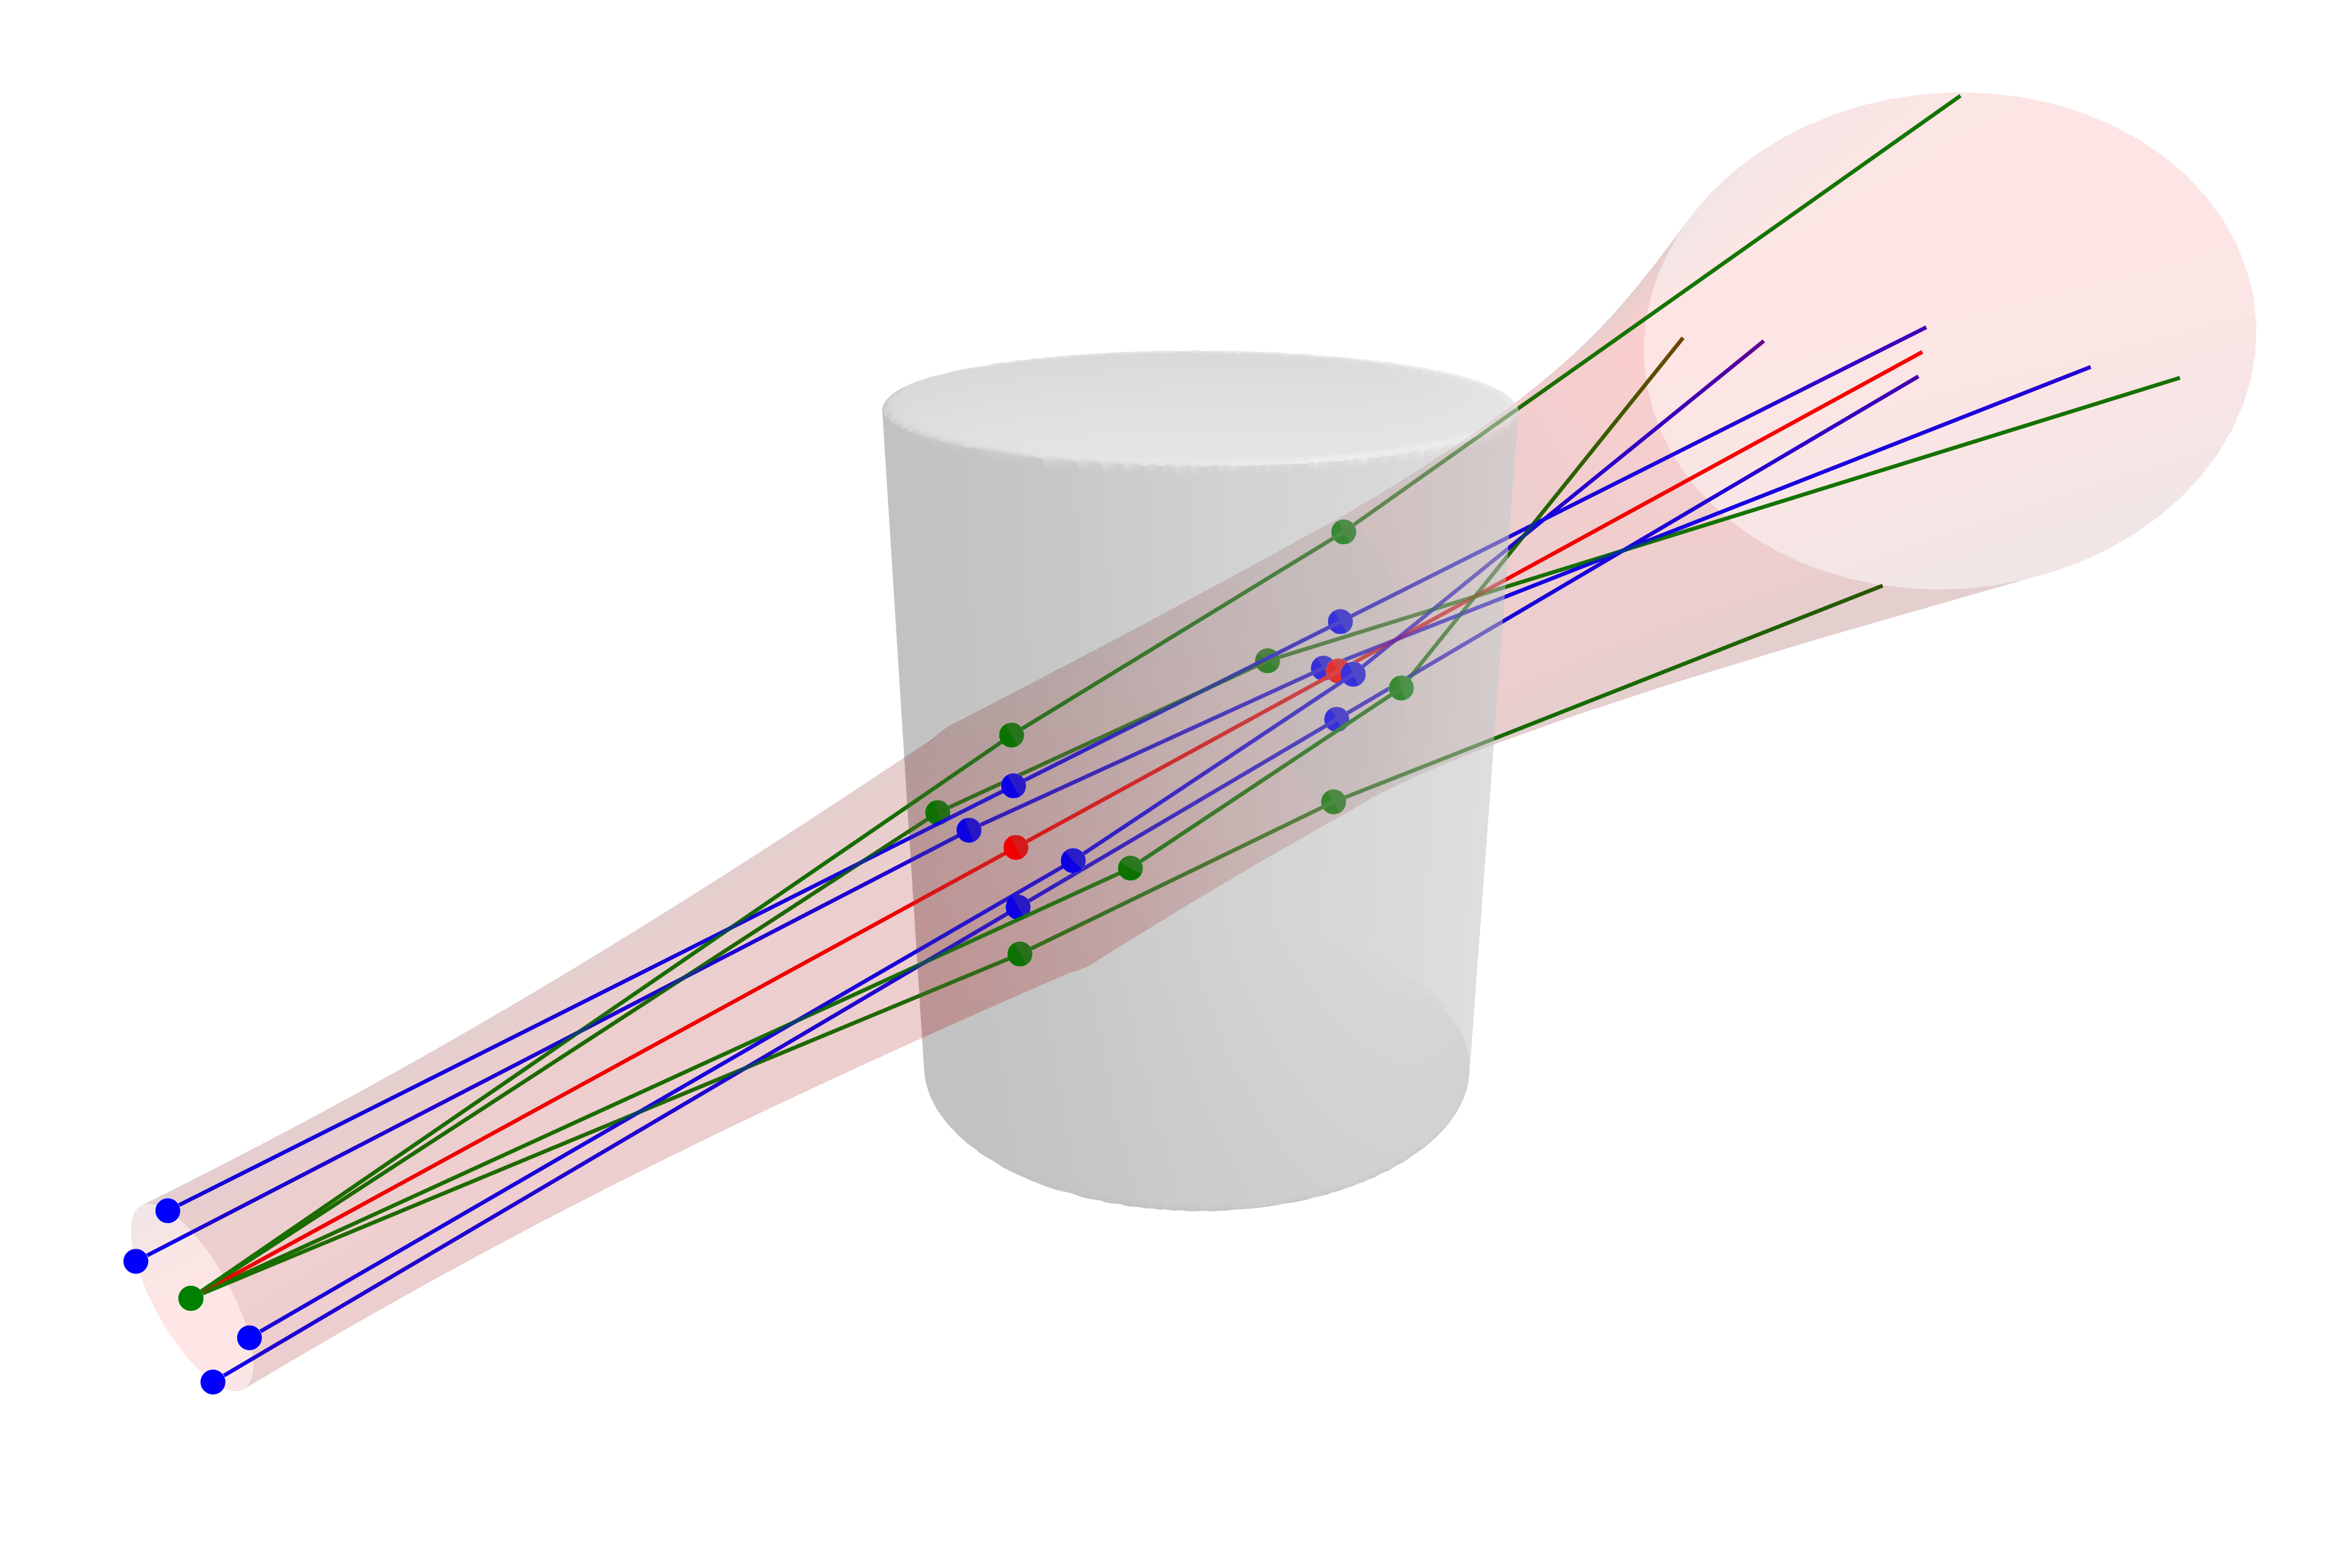
\includegraphics[width=\columnwidth]{figures/agaussian_showcase.png}}
\caption{An \texttt{AstigmaticGaussianBeamlet} passing through a
cylindrical lens. Nine rays sample two orthogonal transverse axes:
polarized chief (red), four waist (blue) and four divergence (green).
The reconstructed envelope is elliptical and the beam acquires the
astigmatism that the three-ray model of Fig.~\ref{fig:beamlet} can not
represent.}
\label{fig:agbeamlet}
\end{figure}

\begin{table}[t]
\tbl{Gaussian beamlet model comparison}{
\begin{tabular}{@{}lll@{}}
\hline
                         & \texttt{GaussianBeamlet} & \texttt{Astigmatic}\ldots \\
\hline
Rays per beamlet         & 3            & 9                     \\
Chief ray type           & \texttt{Ray} & \texttt{PolarizedRay}  \\
Astigmatism              & no           & yes (general)          \\
Higher-order aberrations & no           & no                     \\
Polarization             & no           & yes                    \\
Symmetric systems        & yes          & yes                    \\
Asymmetric systems       & no           & yes                    \\
\hline
\end{tabular}}
\label{tab:models}
\end{table}

\subsection{Beam groups and field decomposition}
\label{sec:beamgroups}

Sources that are not a single mode are built as \emph{beam groups}. For
geometrical ray tracing, the \texttt{CollimatedSource} and
\texttt{PointSource} are initialized as bundles with an equal-area
Fibonacci-sampled spread for correct energy weighting. For beamlet
tracing, decompositions of an arbitrary field into smaller beamlets is
used. The \texttt{GaussianBeamletDecomposition} tiles a larger
$\mathrm{TEM}_{00}$ Gaussian with smaller beamlets for aberration
capture. The \texttt{WavefrontBeamletDecomposition} imports a complex
E-field, e.g. a phase screen or an aperture mask, and maps the local
phase gradient onto a propagation direction per beamlet through the
Eikonal approximation. Because each beamlet is propagated by an exact
ray trace and coherently summed at the detector, this reproduces
diffraction from complex apertures \cite{Greynolds:2014, Ashcraft:2024}.

\section{Available components}

BMO ships a tested library of breadboard components:

\begin{enumerate}
  \item \emph{Mirrors.} Plano mirrors with square, rectangular or round
apertures, plus concave spherical and retroreflector
variants.
  \item \emph{Refractive optics.} Spherical and even-aspheric singlets
through the \texttt{SphericalLens} and \texttt{Lens} constructors,
cemented \texttt{DoubletLens}es, (a)cylindrical lenses and prisms.
  \item \emph{Beamsplitters.} Thin, plate (with an optional
compensator plate) and cube variants.
  \item \emph{Polarizers.} A linear \texttt{PolarizationFilter}, which
acts on the \texttt{PolarizedRay} model of Section~\ref{sec:rays}.
  \item \emph{Non-interacting geometry.} Mounts, tubes and imported
\texttt{.stl} assemblies, added purely for visualization.
\end{enumerate}

Dispersion is modeled in general as a function $n(\lambda)$ for each
refractive element, and is supplied as either a generic Julia function,
a \texttt{DiscreteRefractiveIndex} table or a
\texttt{SellmeierEquation}. Lenses can be specified classically through
an \texttt{AbstractSurface} interface that is internally translated to a
closed SDF volume, so stock catalog parts and published prescriptions
are easy to reproduce, e.g. refer to Fig.~\ref{fig:aspheres}.

In order to investigate optical properties related to the propagation of
beams through a system, the \texttt{Detector} can be used. It consists
of a rectangular 2D screen that accumulates ray or field data during
tracing. From the stored hits it produces \emph{spot diagrams} for a
first geometrical assessment of imaging performance, and \emph{field
distributions} by coherent addition of the ray- or beamlet-attached
fields, i.e. plane waves for geometrical bundles, or Gaussian beam
profiles for beamlets. From these the intensity profile and optical
power can be derived. \texttt{Detector} data is not reset automatically
between solves, so that a kinematic scan can accumulate a signal. The
user calls \texttt{empty!} between runs of \texttt{solve\_system!} to
clear it.

\begin{figure}[h]
\centerline{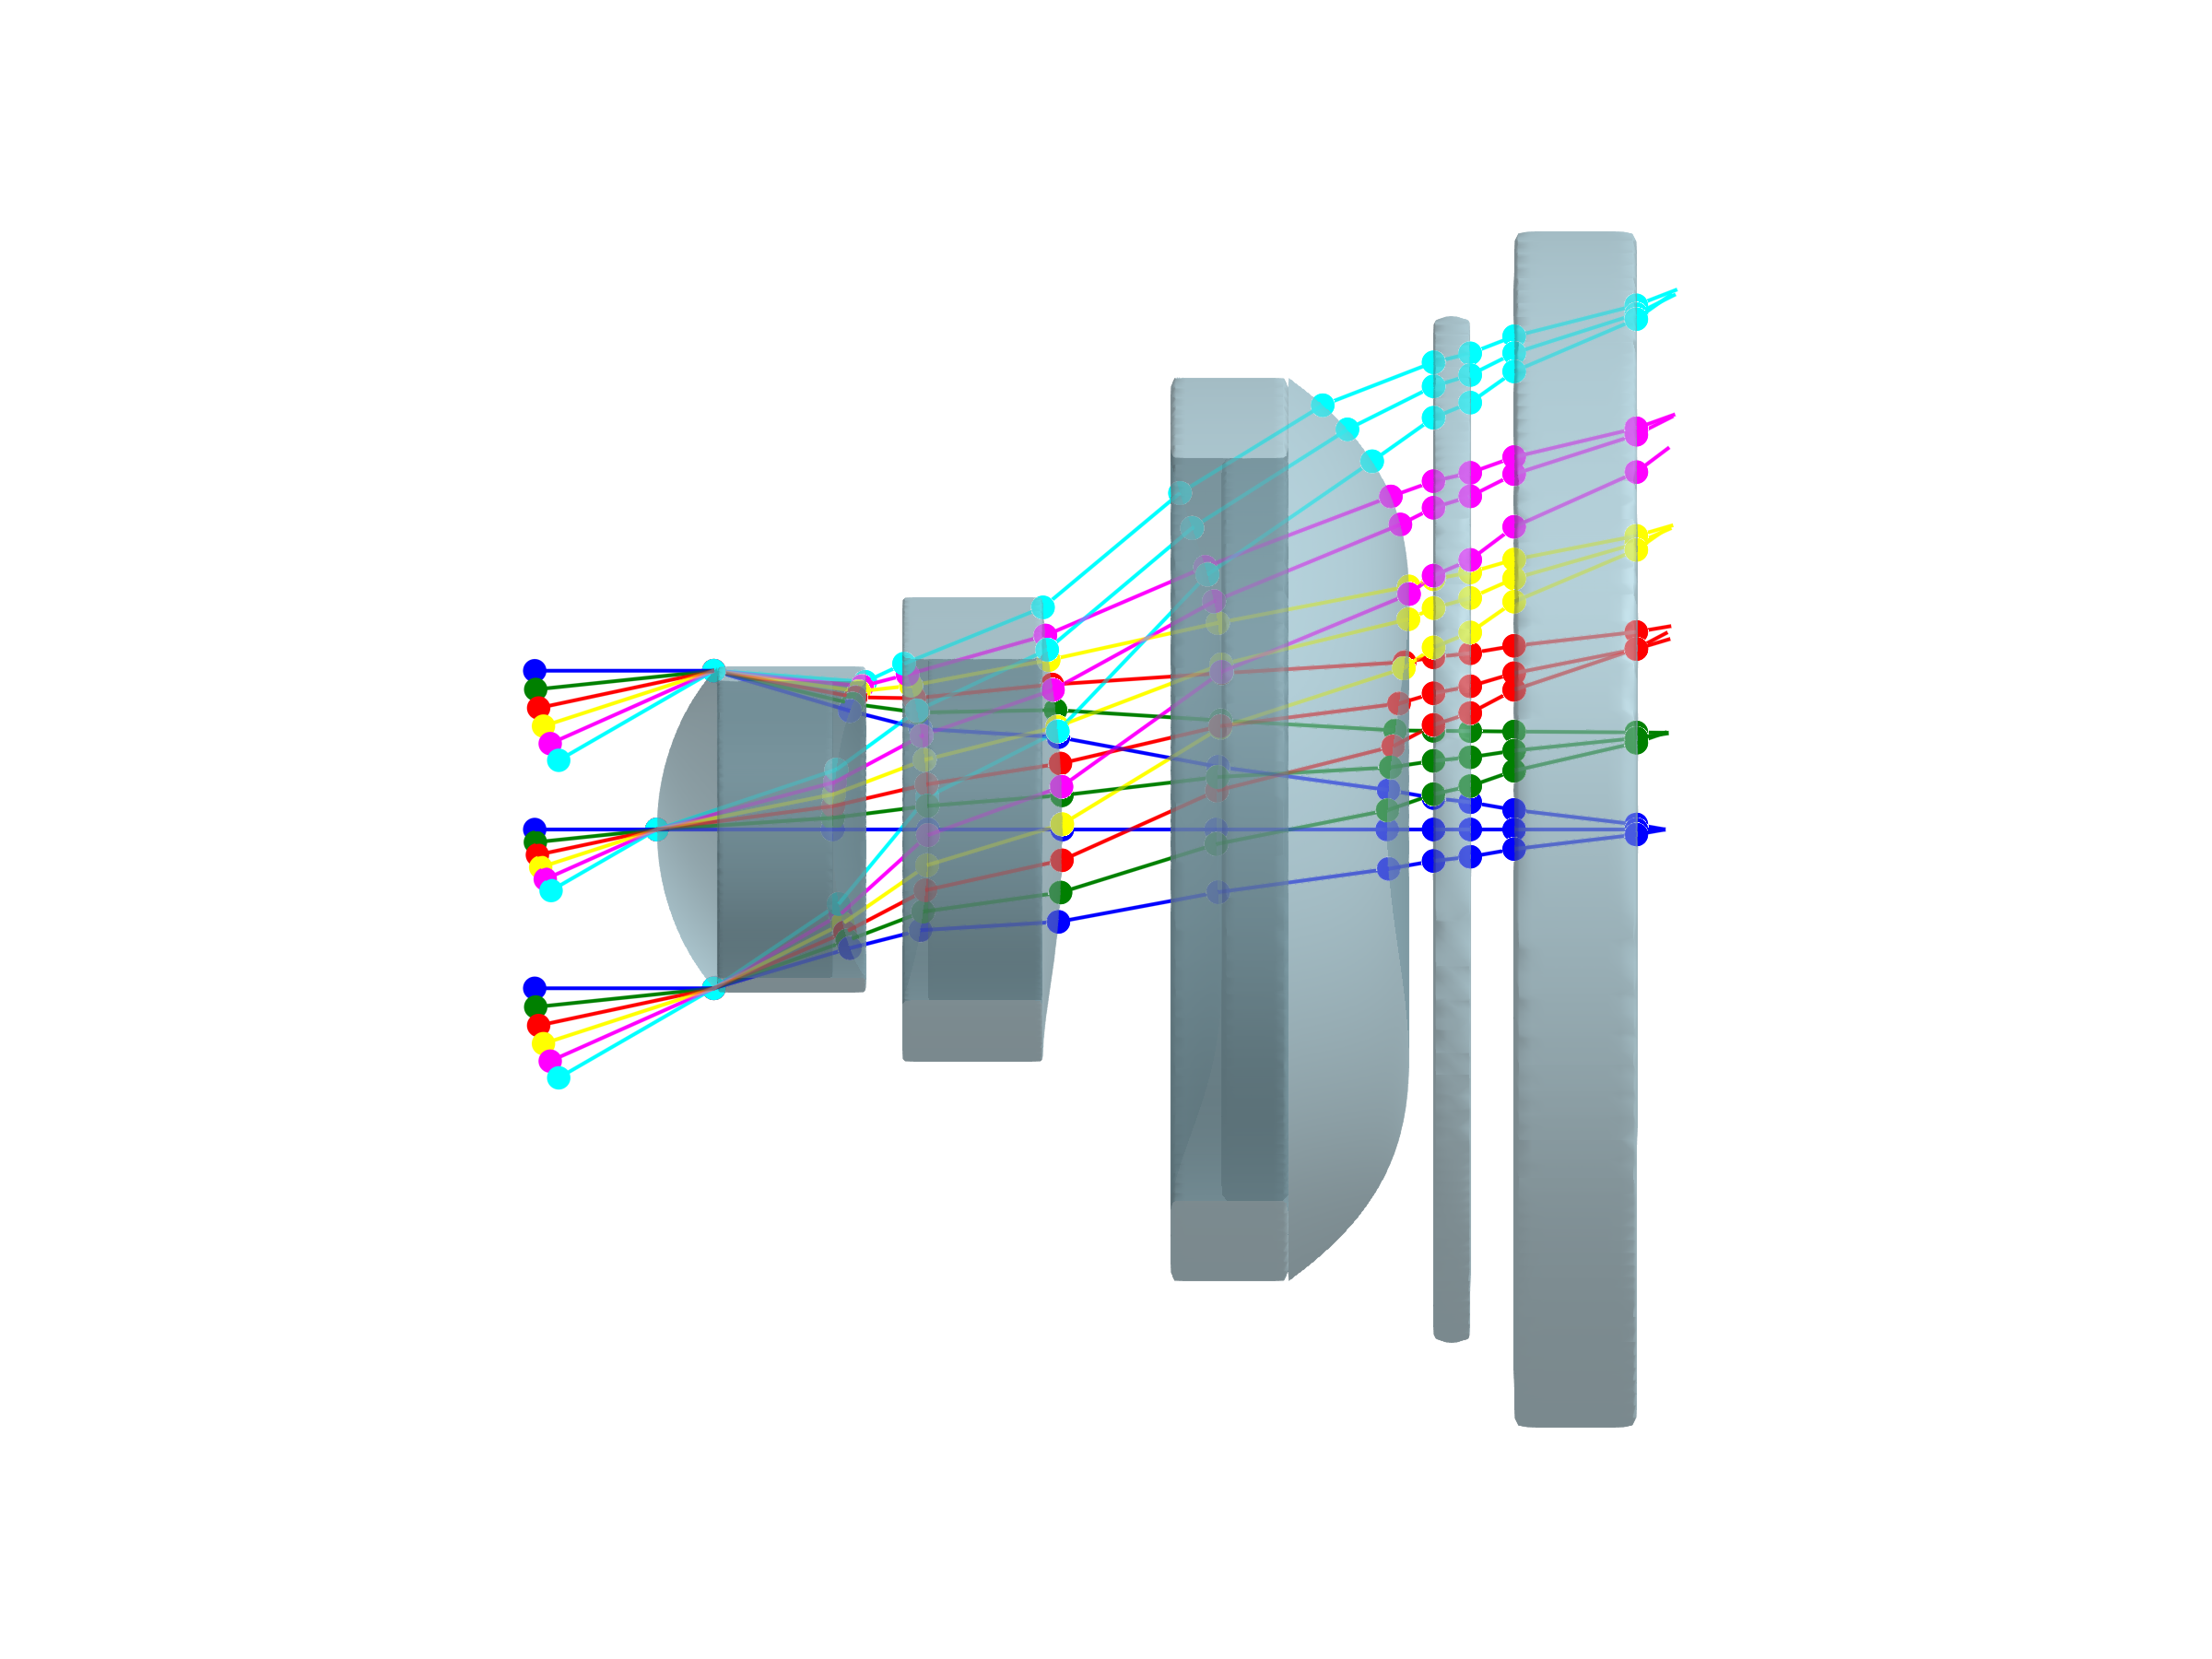
\includegraphics[width=\columnwidth]{figures/mobile_lens.png}}
\caption{A five-element mobile-phone camera objective (even aspheres,
IR filter and cover glass) modeled from a patent prescription
(US8558939). Rays are shown for six field angles up to $30^\circ$.}
\label{fig:aspheres}
\end{figure}

\section{Examples and validation}

\subsection{Michelson interferometer with moving mirror}

A representative application assembles a Michelson interferometer from
stock catalog parts. A \texttt{RightAnglePrismMirror} folds the beam of
a HeNe laser into a 1" \texttt{CubeBeamsplitter}; two
\texttt{RoundPlanoMirror}s return the probe and reference arms, and a
$5\times5$~mm \texttt{Detector} records the recombined field
(Fig.~\ref{fig:michelson}). Cage rods, lens tubes and kinematic mounts
are imported as non-interacting geometry, so the same model doubles as a
mechanical layout check.

\begin{figure}[h]
% trim in bp; the PNG is 4800x4800 px at 768 dpi, i.e. 450x450 bp,
% so 1 bp = 32/3 px. Values below strip the white margin only.
\centerline{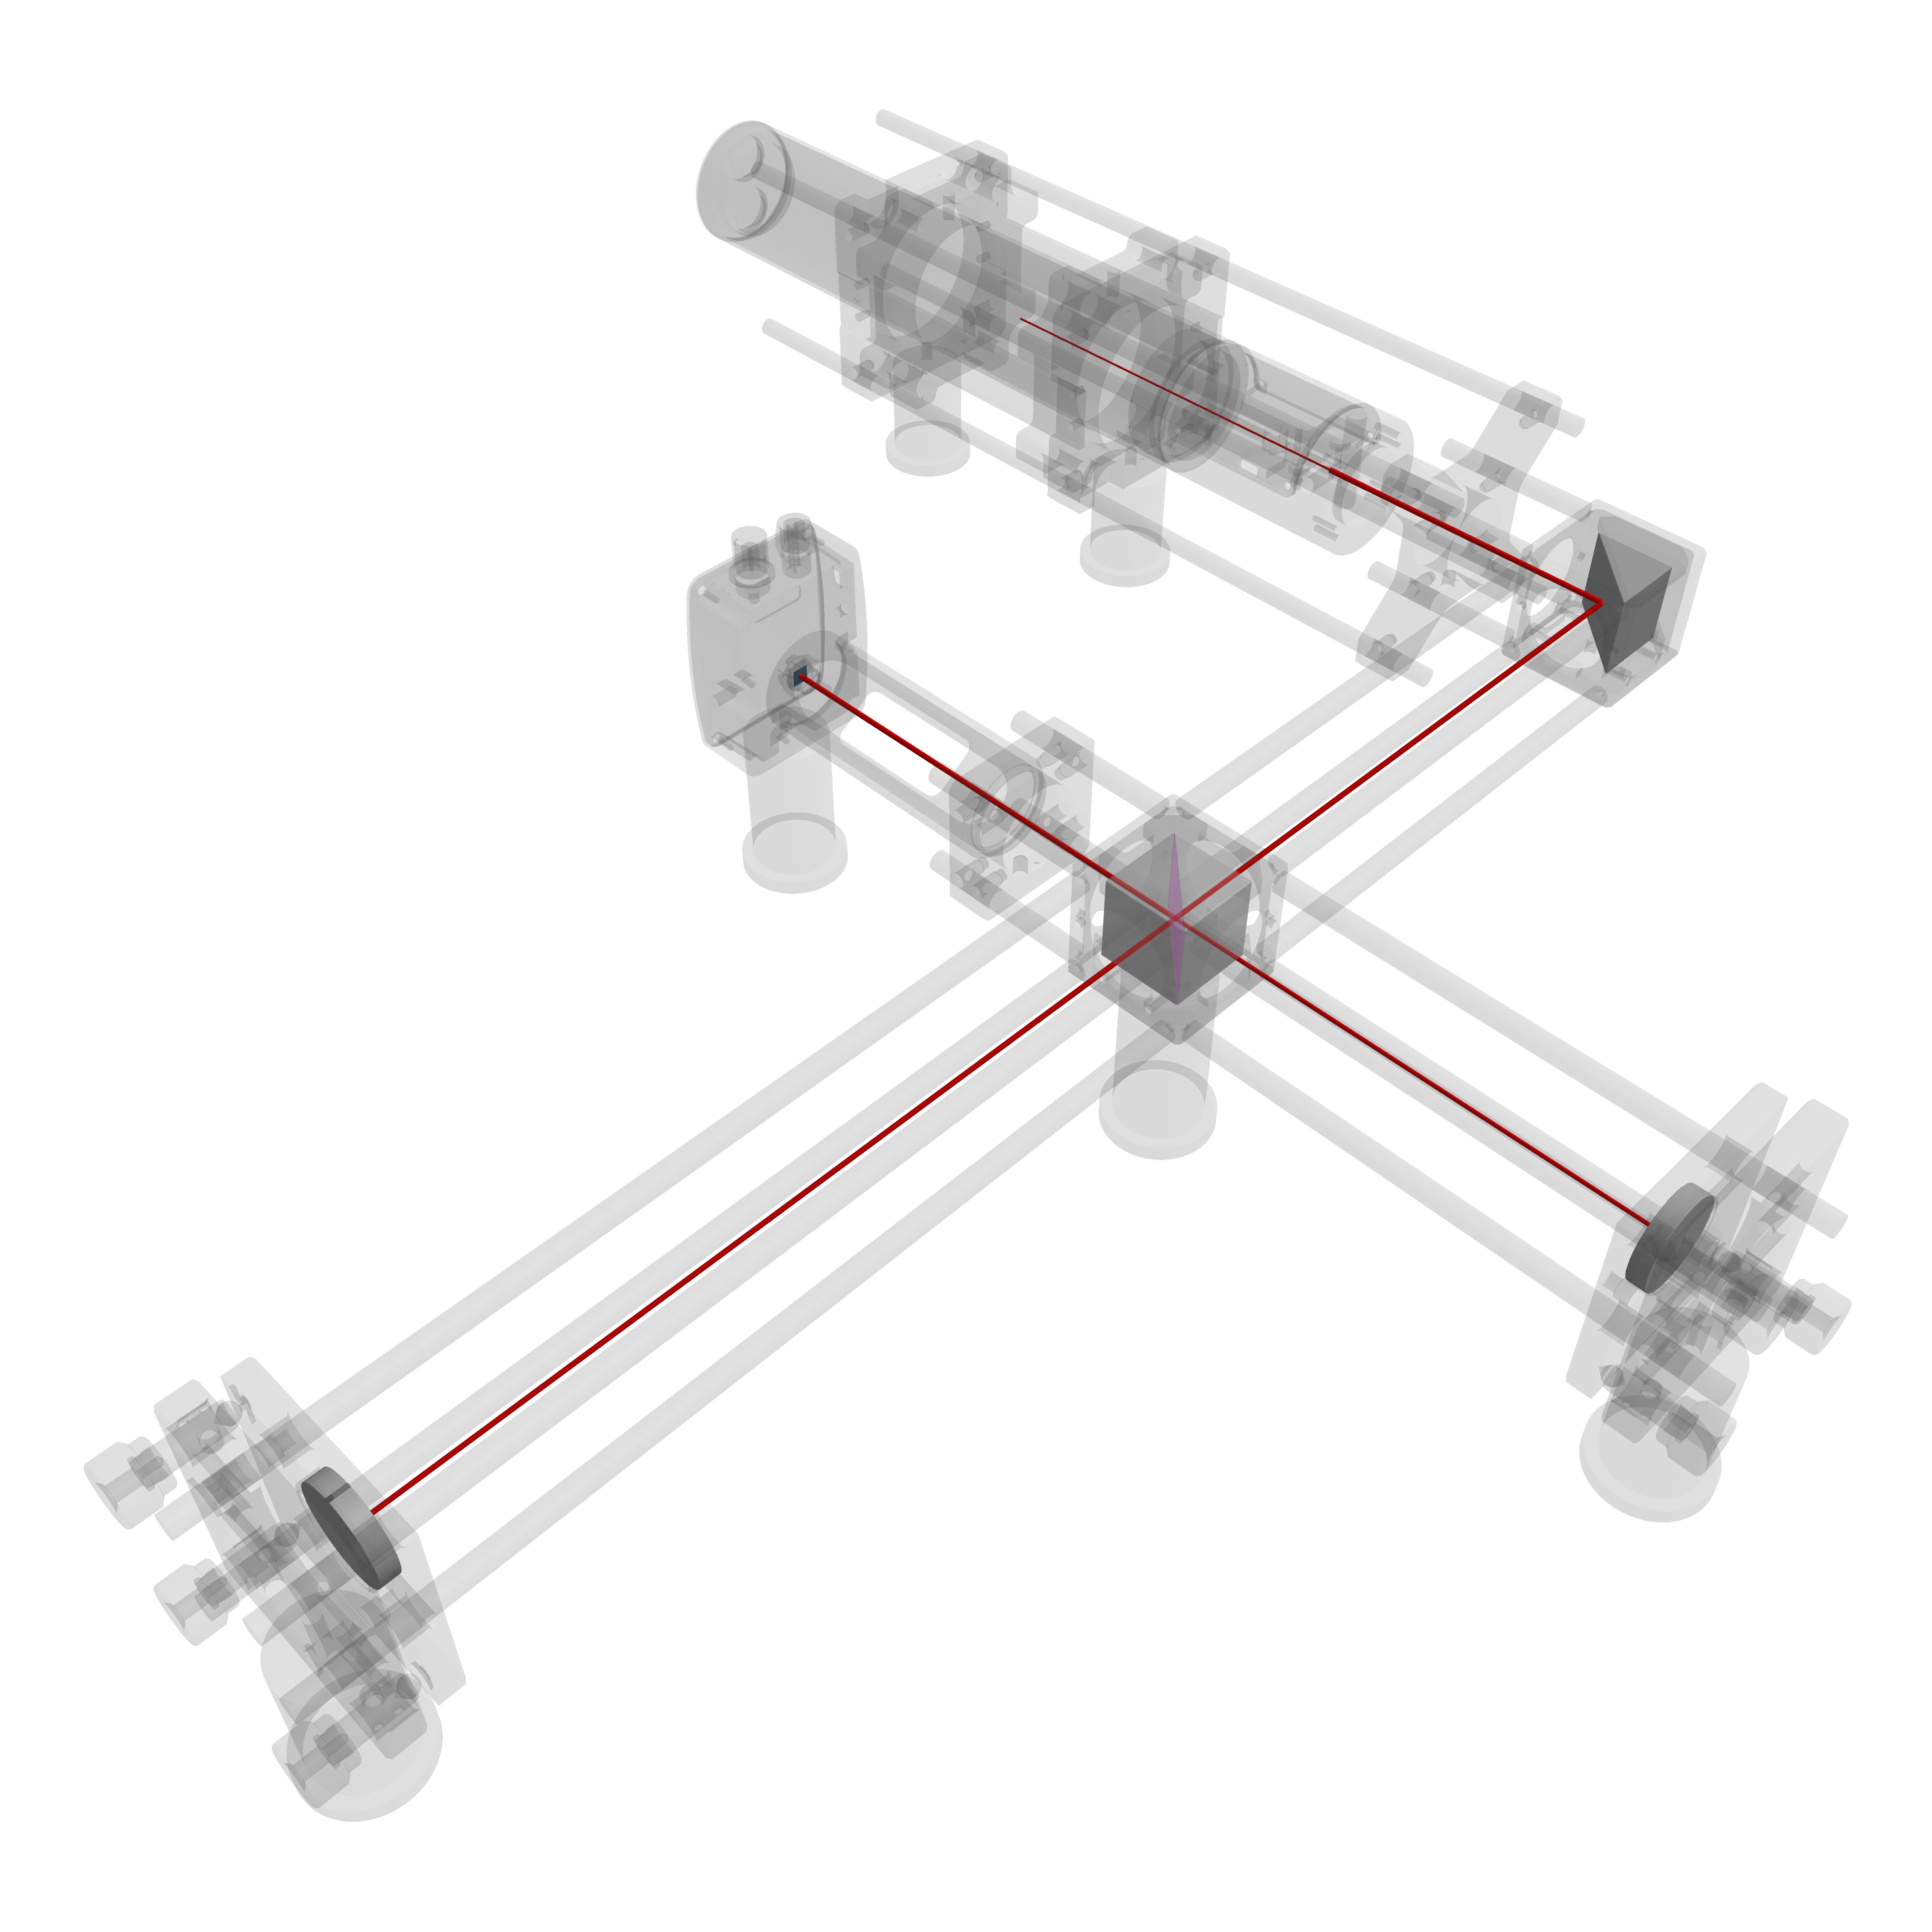
\includegraphics[trim=18 10 6 10, clip,
width=\columnwidth]{figures/michelson_interferometer.png}}
\caption{A Michelson interferometer assembled from catalog components.
The HeNe beam (red) is folded by a right-angle prism mirror into the
cube beamsplitter, retro-reflected by the two end mirrors and recombined
onto the photodetector. Mounts, cage system and lens tubes are
non-interacting mesh geometry. It can also be seen that the beamsplitter
reflects light back into the laser.}
\label{fig:michelson}
\end{figure}

The source is a single \texttt{GaussianBeamlet}. Rather than assume an
ideal mode, its beam-quality factor $M^2$ is recovered from the
divergence figure on the manufacturer's datasheet by inverting
Eq.~\ref{eq:divergence}, which is usually the only mode information a
laser datasheet provides (Code~\ref{lst:hene}).

\begin{lstlisting}[
  language = Julia,
  numbers = left,
  label = {lst:hene},
  caption = {Defining a HeNe source as a Gaussian beamlet with a 
  beam-quality factor.} 
]
  lambda = 632.8e-9
  w0 = 0.65e-3 / 2 # waist radius
  theta_spec = 1.4e-3 / 2 # spec. half-angle
  theta_ideal = divergence_angle(lambda, w0, 1)
  M2 = theta_spec / theta_ideal
  beam = GaussianBeamlet(
    [0.0, 0.0, 0.0], # origin 
    [0.0, 1.0, 0.0], # y = optical axis 
    lambda, w0; M2)
\end{lstlisting}

Because every element is movable, the experiment itself is a loop over
\texttt{solve\_system!} calls, with components repositioned between
calls to produce the intended effect. With the interferometer aligned,
one end mirror is translated along its own axis in $\lambda/100$ steps
and the power on the detector is integrated at each step, which yields
an optical power curve as a function of displacement
(Fig.~\ref{fig:mipower}). Two full periods appear over one wavelength of
mirror travel, because the light crosses that arm twice and a
displacement $\Delta y$ therefore changes the path difference by
$2\,\Delta y$. The interferometric phase is therefore
\begin{equation}
\varphi = \frac{4\pi\,\Delta y}{\lambda},
  \label{eq:miphase}
\end{equation}
and, at an ideal fringe contrast $V = 1$, the recombined power on the
detector follows
\begin{equation}
P = P_\mathrm{in}\,\cos^2\!\left(\frac{\varphi}{2}\right).
  \label{eq:mipower}
\end{equation}
The simulated curve reaches neither zero nor the full 1~mW of the
source, peaking at 0.985~mW and dipping to 0.012~mW ($V = 0.975$): the
two arms are not exactly equal in length, so the recombined beams have
slightly different radii and curvatures on the detector and do not
interfere perfectly. This simulation pattern --- move a component,
solve, read the detector --- is the outer loop of Fig.~\ref{fig:iir},
and is the basis of BMO's use in modeling e.g. sensitivity to
vibrations; see the master's thesis of Manny \cite{Manny:2024} for a
detailed treatment.


\begin{figure}[h]
\centerline{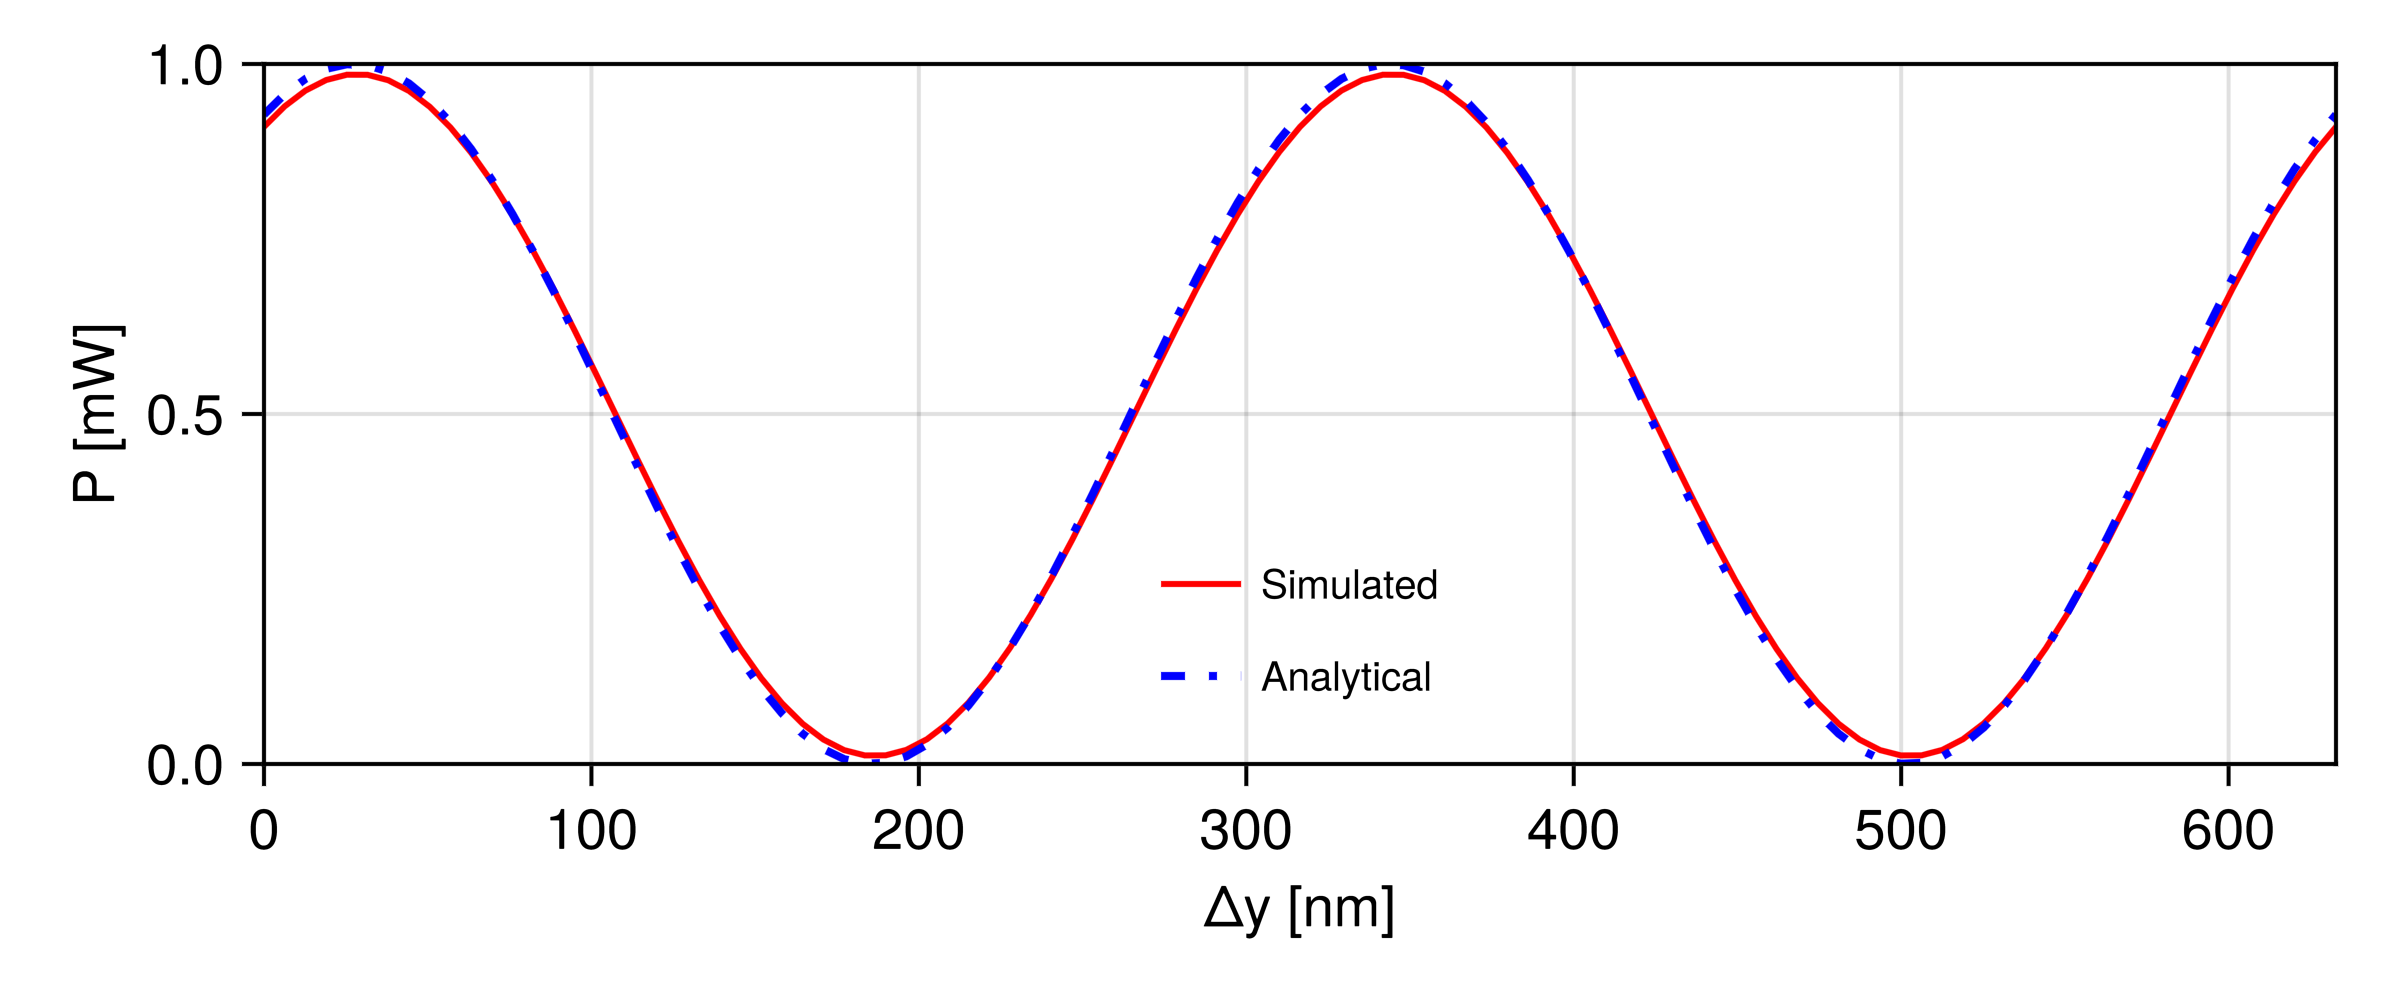
\includegraphics[width=\columnwidth]{figures/michelson_powerplot.png}}
\caption{Optical power on the photodetector (red) as one end mirror is
translated by one wavelength $\lambda$, marked by the vertical
dash-dotted line. The blue dash-dotted curve is the analytical
prediction of Eq.~\ref{eq:mipower} at ideal fringe contrast $V = 1$;
only its phase offset is taken from the simulation, while period and
contrast are purely analytical. The two periods per $\lambda$ follow
from the path difference changing by $2\,\Delta y$; the non-zero minimum
and sub-unity maximum of the simulated curve reflect the slight
arm-length imbalance.}
\label{fig:mipower}
\end{figure}

\subsection{Fraunhofer diffraction from a double slit}

To validate the astigmatic beamlet model against wave optics, a classic
double slit (slit width $a = 10$~\textmu{}m, pitch $d = 100$~\textmu{}m,
$\lambda = 633$~nm) is written as an amplitude mask, decomposed with
\texttt{WavefrontBeamletDecomposition} into a few thousand coherent
beamlets, and propagated $L = 0.2$~m to a detector. At that distance the
screen is in the far field, where scalar diffraction theory predicts the
two-slit interference term modulated by the single-slit envelope
\cite{Goodman2005},
\begin{equation}
I(x) = I_0\, \operatorname{sinc}^2\!\left(\frac{\pi a x}{\lambda
L}\right) \cos^2\!\left(\frac{\pi d x}{\lambda L}\right),
  \label{eq:fraunhofer}
\end{equation}
with $\operatorname{sinc}(u) = \sin(u)/u$. Every beamlet produced by the
decomposition is traced geometrically and the beamlet fields are summed
coherently on the detector. The resulting cross-section follows
Eq.~\ref{eq:fraunhofer} fringe for fringe (Fig.~\ref{fig:doubleslit}),
reproducing both the fringe spacing $\lambda L / d = 1.27$~mm and the
first envelope zero at $\lambda L / a = 12.7$~mm. Because $d/a = 10$
exactly, the two coincide: the tenth interference order falls on the
envelope zero and is suppressed, which the traced result reproduces as
well.

\begin{figure}[h]
\centerline{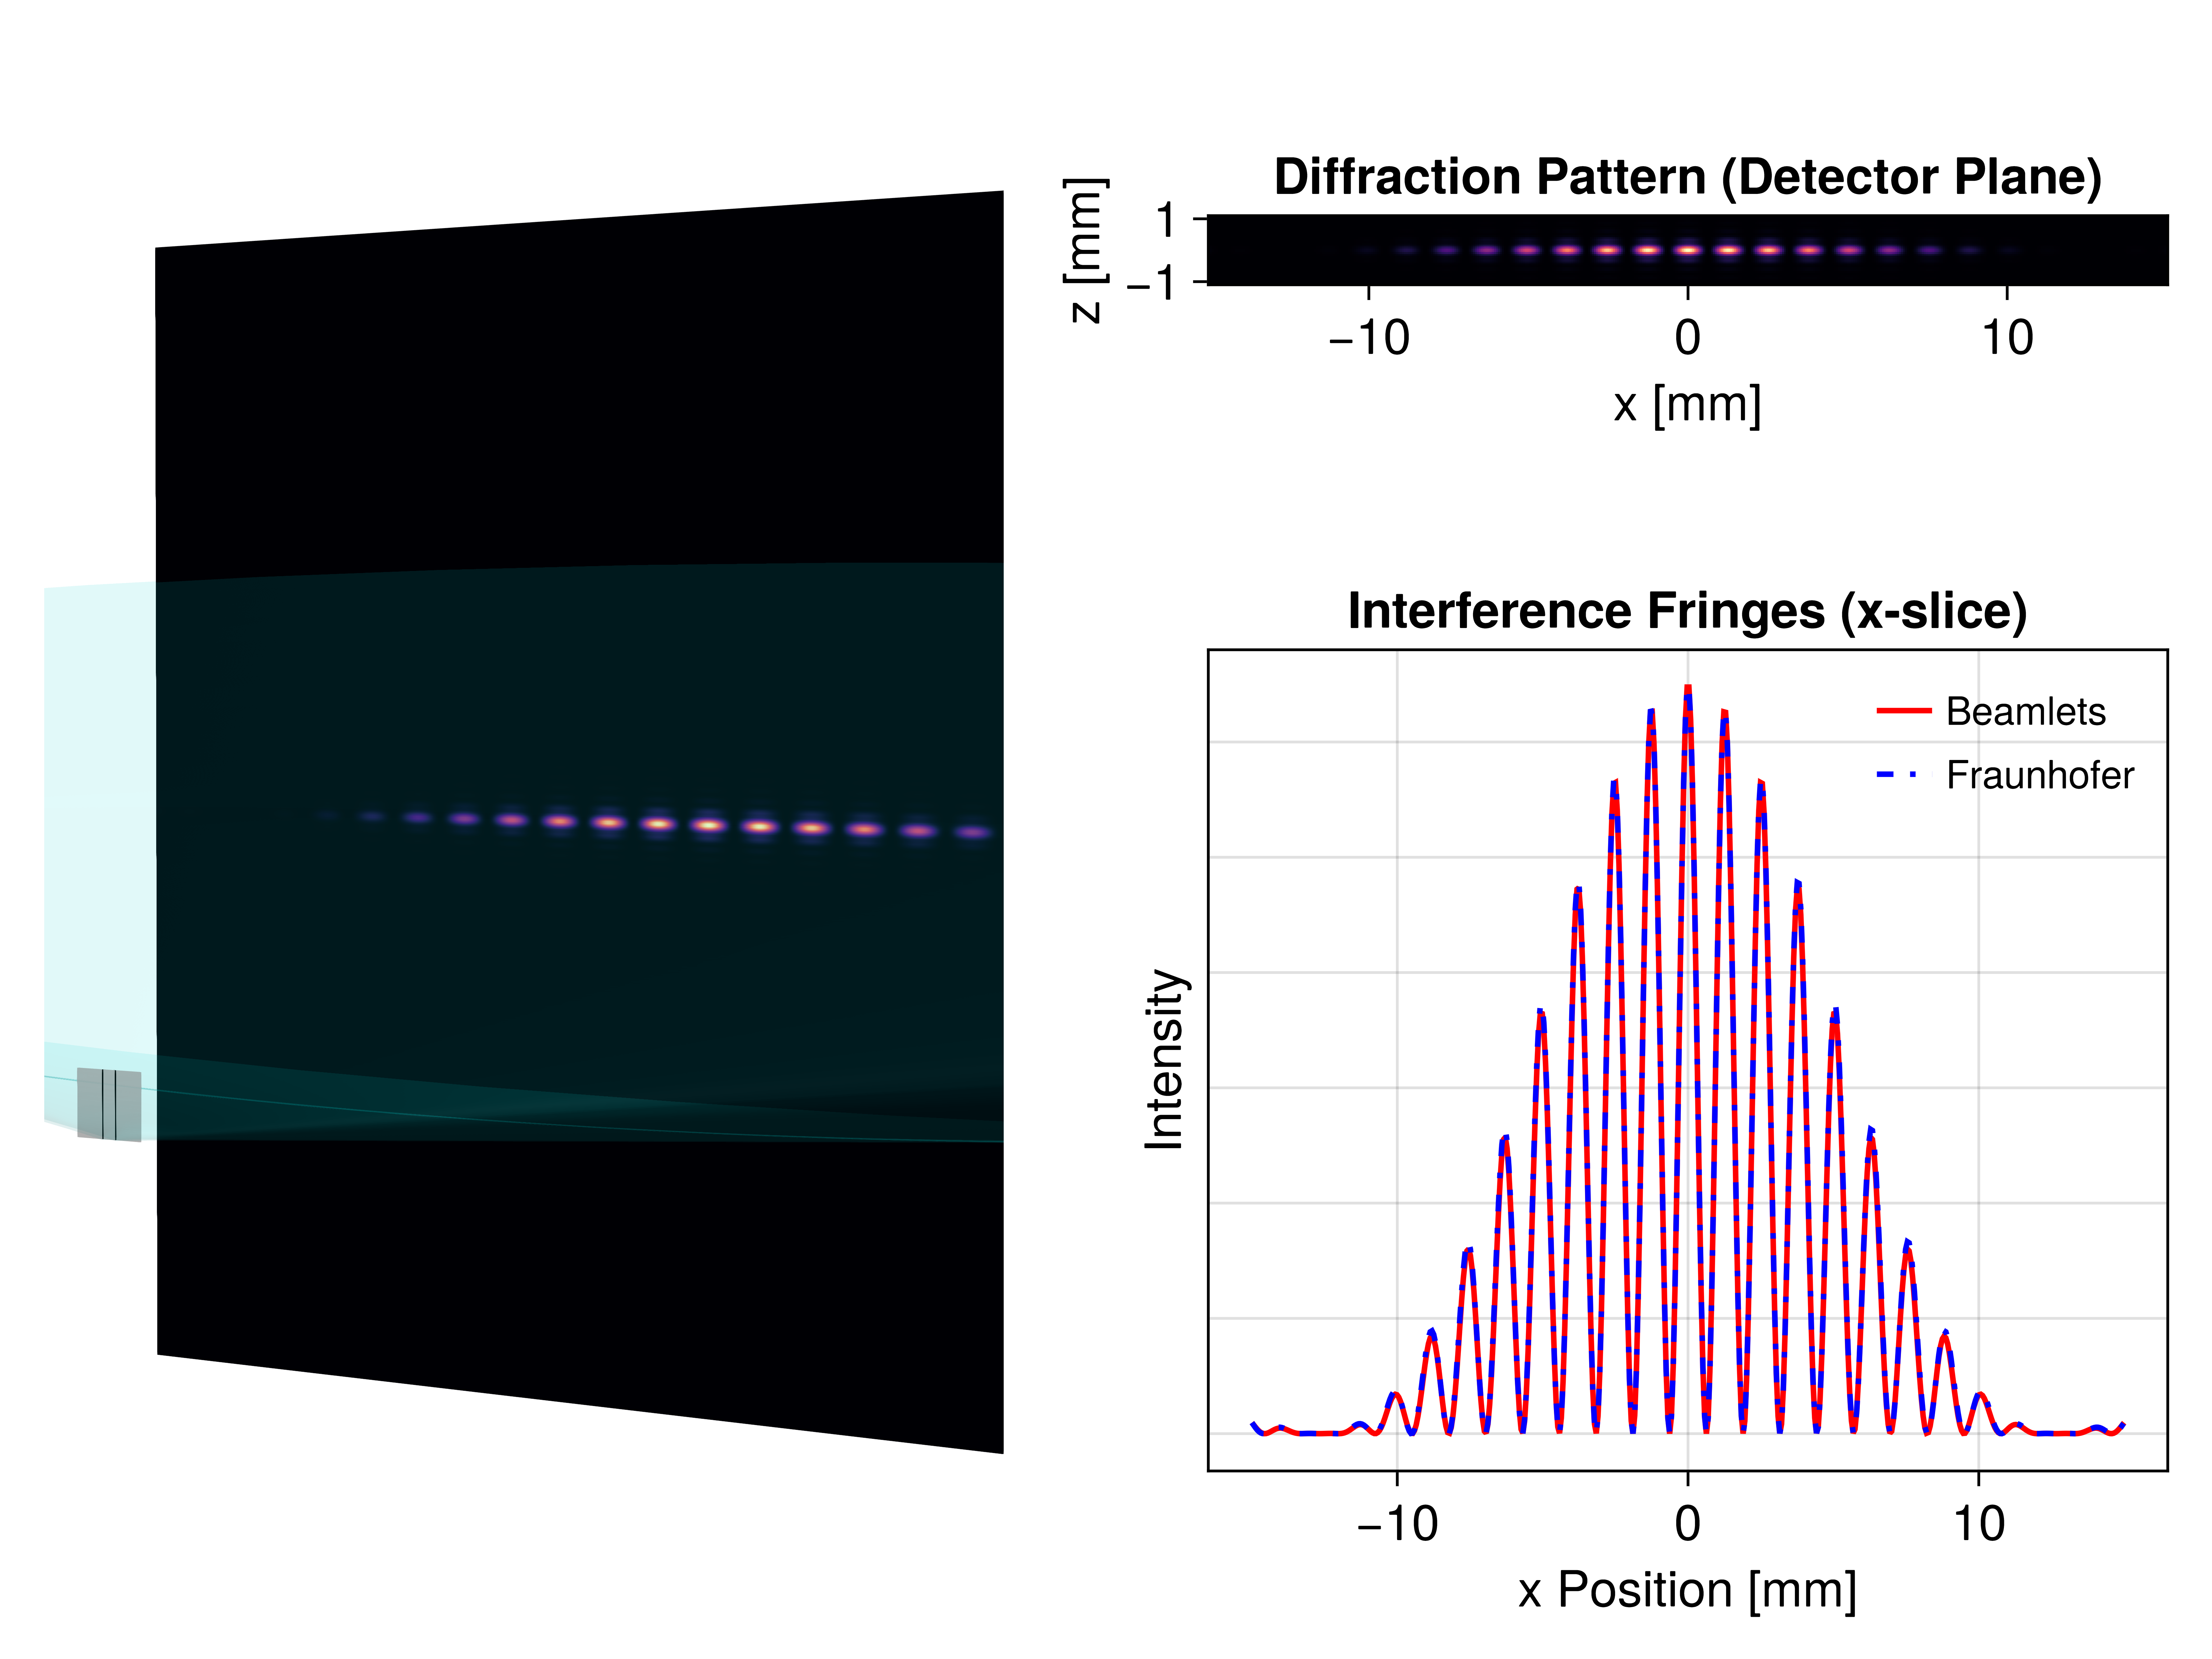
\includegraphics[width=\columnwidth]{figures/agb_doubleslit.png}}
\caption{Double-slit diffraction by coherent beamlet decomposition.
Left: the amplitude mask (grey) and the beamlet bundle propagating to
the screen, on which the fringes are visible. Top right: intensity in
the detector plane. Bottom right: the central cross-section traced by
BMO (red) against the analytical Fraunhofer prediction of
Eq.~\ref{eq:fraunhofer} (blue, dashed).}
\label{fig:doubleslit}
\end{figure}

\subsection{Performance notes}

The computational cost of tracing a system is dominated by the
intersection tests, which currently scale by $\mathcal{O}(n)$ with the number $n$ of
intersectable objects. We have not yet benchmarked BMO against
comparable software, since we still see room for improvement through
more sophisticated tracing methods, e.g. sphere-of-influence testing.
Further, the current implementations of \texttt{solve\_system!} for the
geometrical beams and Gaussian beamlets rely on branching logic, which
makes GPU adaptation difficult; as of version 0.13, all tracing
algorithms run on the CPU. Tracing a system is deliberately
separated from the evaluation of field data, so that the computationally
expensive calculation of field distributions can be triggered outside of
the solver loop, at a point of the user's choosing.

\section{Limitations and roadmap}

BMO is pre-1.0 and its scope is deliberately narrow. It does not
optimize optical systems, model coatings or partial coherence, or handle
hard-aperture clipping of beamlets rigorously. As noted in the previous
section, the solver is a branching CPU algorithm with no GPU backend.
The near-term roadmap targets additional polarizing optics (wave plates,
retarders, Faraday rotators) built on the Jones and 3D polarization
calculus of Section~\ref{sec:rays}, modulators (AOM/EOM),
coherence-length and contrast modeling, and interactive Makie updates.
We also anticipate breaking internal API changes in order to introduce more
sophisticated boundary-interaction handling.

\section{Conclusion}

BeamletOptics.jl provides a practical, open-source environment for
prototyping three-dimensional breadboard optical setups with laser
sources in Julia. By tracing the fundamental Gaussian mode as a small
bundle of exact geometrical rays through closed, SDF- and mesh-defined volumes,
and by keeping every component freely movable, it bridges the gap
between paraxial $ABCD$ tools and heavyweight commercial design suites.
The implementation is validated against analytical diffraction results,
and is in active use for laser interferometer modeling at the Institute
of Technical Physics (DLR). Future work will aim to build better tooling
and to improve the solver architecture, in order to allow for more
modeling capability, e.g. coatings or inhomogeneous media with curved
ray paths.

\section*{Acknowledgements}

We thank the JuliaPhysics organization for hosting the package and
Brian Guenter for valuable technical discussions. We thank Thorsten \"Osterle
for proof-reading the manuscript. BeamletOptics.jl builds on the Julia language
\cite{bezanson2017julia} and the Makie visualization ecosystem
\cite{Danisch2021}.

\section*{Disclosures}

During the preparation of this manuscript, the authors used \mbox{Opus 5
(Anthropic)} for grammar and spelling correction, formatting support,
and consistency checks of notation, terminology, and cross-references.
No results, figures or arguments were generated by AI. The authors
reviewed and edited all output and take full responsibility for the
content of the publication.

\input{bib.tex}

\end{document}
